\documentclass{article} % For LaTeX2e
\usepackage{iclr2018_conference,times}
 % \usepackage{hyperref}
\usepackage{url}

\usepackage[T1]{fontenc}  
\usepackage[utf8]{inputenc}             
 % \usepackage[english,french]{babel}  
\usepackage[english]{babel} 

\usepackage{graphicx}
\usepackage{caption}
\usepackage{booktabs}
\usepackage{enumitem}

\usepackage{amsmath}
\usepackage{amsfonts}
\usepackage{amsthm}

\newcommand*\samethanks[1][\value{footnote}]{\footnotemark[#1]}

\title{Breaking the Softmax Bottleneck: \\ A High-Rank RNN Language Model}

% Authors must not appear in the submitted version. They should be hidden
% as long as the \iclrfinalcopy macro remains commented out below.
% Non-anonymous submissions will be rejected without review.

\author{Zhilin Yang\thanks{Equal contribution. Ordering determined by dice rolling.}~~, Zihang Dai\samethanks~~, Ruslan Salakhutdinov, William W. Cohen\\
School of Computer Science\\
Carnegie Mellon University\\
\texttt{\{zhiliny,dzihang,rsalakhu,wcohen\}@cs.cmu.edu}
}

% The \author macro works with any number of authors. There are two commands
% used to separate the names and addresses of multiple authors: \And and \AND.
%
% Using \And between authors leaves it to \LaTeX{} to determine where to break
% the lines. Using \AND forces a linebreak at that point. So, if \LaTeX{}
% puts 3 of 4 authors names on the first line, and the last on the second
% line, try using \AND instead of \And before the third author name.

% table cell
\usepackage{array}
\newcolumntype{C}{>{\centering\arraybackslash}p{0.15\linewidth}}

% table cell length
\newlength\contextlength 
\setlength\contextlength{\linewidth}

% special token
\newcommand{\blank}{\_\_?\_\_}

\newcommand{\fix}{\marginpar{FIX}}
\newcommand{\new}{\marginpar{NEW}}
\newcommand{\todo}[1]{{\color{red} TODO: {#1}}}

\iclrfinalcopy % Uncomment for camera-ready version, but NOT for submission.

\newtheorem{lemma}{Lemma}
\newtheorem{prop}{Proposition}
\newtheorem{coro}{Corollary}
\newtheorem{property}{Property}

\begin{document}


\maketitle

\begin{abstract}
We formulate language modeling as a matrix factorization problem, and show that the expressiveness of Softmax-based models (including the majority of neural language models) is limited by a {\em Softmax bottleneck}. Given that natural language is highly context-dependent, this further implies that in practice Softmax with distributed word embeddings does not have enough capacity to model natural language. We propose a simple and effective method to address this issue, and improve the state-of-the-art perplexities on Penn Treebank and WikiText-2 to 47.69 and 40.68 respectively. The proposed method also excels on the large-scale 1B Word dataset, outperforming the baseline by over 5.6 points in perplexity.\footnote{Code is available at \url{https://github.com/zihangdai/mos}.}
\end{abstract}


%\cite{burger2001issues}
%\cite{fader2014open}
%\cite{voorhees1999trec}


%A huge leap forward in artificial intelligence will be achieved when
%machines will be able to answer any question expressed in natural
%language. As such, q

Question answering (QA) has been a long standing research problem in
natural language processing, with the first systems attempting to
answer questions by directly reading
documents \citep{voorhees2000building}. The development of large-scale Knowledge Bases (KBs) such as Freebase  \citep{bollacker2008freebase}
helped organize information into structured forms, prompting recent progress to focus on answering questions by converting them into logical forms that can be used to query such databases \citep{berant2013semantic,kwiatkowski-EtAl:2013:EMNLP,fader2014open}.

Unfortunately, KBs have intrinsic limitations such as their inevitable incompleteness and fixed schemas that cannot support all varieties of answers.
%
Since information extraction (IE) \citep{craven2000learning}, intended to
fill in missing information in KBs, is neither accurate nor
reliable enough, collections of raw textual resources and
documents such as Wikipedia will always contain more information.
%than KBs.
%
As a result, even if KBs can be satisfactory for closed-domain problems, they are unlikely
to scale up to answer general questions on any
topic.
%
Starting from this observation,
%here we propose  to study the problem
in this work we study the problem
of answering by directly reading documents.


Retrieving answers directly from text is harder than
from KBs because information is far less structured, is
indirectly and ambiguously expressed, and is usually scattered across multiple documents.
%
%This explains why, when a satisfactory KB is
%available -- which is typically only the case in closed domains --
%using it instead of raw text is preferred. %, because performance is better.
%
This explains why using a satisfactory KB---typically only available in closed domains---is preferred over raw text.
%
We postulate that before trying to provide answers that are not in
KBs, document-based QA systems should first reach KB-based systems'
performance in such closed domains, where clear comparison and
evaluation is possible.
%
To this end, this paper introduces {\sc WikiMovies}, a new
analysis tool that allows for measuring the performance of %loss induced on
QA systems when the knowledge source is switched from a KB to unstructured documents.
%
{\sc WikiMovies} contains $\sim$100k questions in the movie domain, and was designed
to be answerable by using either a perfect KB
(based on OMDb\footnote{\url{http://www.omdbapi.com}}), Wikipedia pages or an imperfect KB obtained through
running %a standard IE pipeline on those pages.
an engineered IE pipeline on those pages.

To bridge the gap between using a KB and reading documents directly,
we still lack appropriate machine learning algorithms. In this
work we propose the Key-Value Memory Network (KV-MemNN), a new neural network
architecture that generalizes the original Memory Network
\citep{sukhbaatar2015end} and can work with either knowledge source.
%
The KV-MemNN performs QA by first storing facts in a key-value
structured memory before reasoning on them in order to predict an
answer. The memory is designed so that the model learns to use keys to
address relevant memories with respect to the question, whose corresponding values are subsequently returned.
%
This structure allows the model to encode prior knowledge for the considered task
and to leverage possibly complex transforms between keys and values,
while still being trained using standard backpropagation via
stochastic gradient descent.

Our experiments on {\sc WikiMovies} indicate that, thanks to its key-value memory,
the KV-MemNN consistently outperforms the
original Memory Network, and reduces the gap between answering from a human-annotated KB,
from an automatically extracted KB or from directly reading Wikipedia.
%
We confirm our findings on  {\sc WikiQA} \citep{yang2015wikiqa},
another Wikipedia-based QA benchmark where no KB is available,
where we demonstrate that KV-MemNN can reach state-of-the-art results---surpassing
the most recent attention-based neural network models.


\section{Language Modeling as Matrix Factorization}\label{sec:rank}

As discussed in Section \ref{sec:intro}, with the autoregressive factorization, language modeling can be reduced to modeling the conditional distribution of the next token $x$ given the context $c$. Though one might argue that a natural language allows an infinite number of contexts due to its compositionality \citep{pinker1994language}, we proceed with our analysis by considering a finite set of possible contexts. The unboundedness of natural language does not affect our conclusions, which will be discussed later.

We consider a natural language as a finite set of pairs of a context and its conditional next-token distribution\footnote{We use capital letters for variables and small letters for constants.} $\mathcal{L} = \{(c_1, P^*(X | c_1)), \cdots, (c_N, P^*(X | c_N))\}$, where $N$ is the number of possible contexts. We assume $P^* > 0$ everywhere to account for errors and flexibility in natural language. Let $\{x_1, x_2, \cdots, x_M\}$ denote a set of $M$ possible tokens in the language $\mathcal{L}$. The objective of a language model is to learn a model distribution $P_\theta(X | C)$ parameterized by $\theta$ to match the true data distribution $P^*(X | C)$.

In this work, we study the expressiveness of the parametric model class $P_\theta(X | C)$.
In other words, we are asking the following question: given a natural language $\mathcal{L}$, does there exist a parameter $\theta$ such that $P_\theta(X | c) = P^*(X | c)$ for all $c$ in $\mathcal{L}$?

We start by looking at a Softmax-based model class since it is widely used.

\subsection{Softmax}

The majority of parametric language models use a Softmax function operating on a context vector (or hidden state) $\mathbf{h}_c$ and a word embedding $\mathbf{w}_x$ to define the conditional distribution $P_\theta(x | c)$. More specifically, the model distribution is usually written as
\begin{equation}\label{eqn:softmax}
P_\theta(x | c) = \frac{\exp \mathbf{h}^\top_c \mathbf{w}_x}{\sum_{x'} \exp \mathbf{h}^\top_c \mathbf{w}_{x'}}
\end{equation}
where $\mathbf{h}_c$ is a function of $c$, and $\mathbf{w}_x$ is a function of $x$. Both functions are parameterized by $\theta$. Both the context vector $\mathbf{h}_c$ and the word embedding $\mathbf{w}_x$ have the same dimension $d$. The dot product $\mathbf{h}_c^\top \mathbf{w}_x$ is called a {\em logit}.

To help discuss the expressiveness of Softmax, we define three matrices:
\[
\mathbf{H}_\theta = \begin{bmatrix}
\mathbf{h}_{c_1}^\top \\
\mathbf{h}_{c_2}^\top \\
\cdots \\
\mathbf{h}_{c_N}^\top
\end{bmatrix}; ~~
\mathbf{W}_\theta = \begin{bmatrix}
\mathbf{w}_{x_1}^\top \\
\mathbf{w}_{x_2}^\top \\
\cdots \\
\mathbf{w}_{x_M}^\top
\end{bmatrix}; ~~
\mathbf{A} = \begin{bmatrix}
\log P^* (x_1 | c_1),& \log P^* (x_2 | c_1)& \cdots& \log P^*(x_M | c_1) \\
\log P^* (x_1 | c_2),& \log P^* (x_2 | c_2)& \cdots& \log P^* (x_M | c_2) \\
\vdots& \vdots& \ddots& \vdots \\
\log P^* (x_1 | c_N),& \log P^* (x_2 | c_N)& \cdots& \log P^* (x_M | c_N)
\end{bmatrix}
\]
where $\mathbf{H}_\theta \in \mathbb{R}^{N \times d}$, $\mathbf{W}_\theta \in \mathbb{R}^{M \times d}$, $\mathbf{A} \in \mathbb{R}^{N \times M}$, and the rows of $\mathbf{H}_\theta$, $\mathbf{W}_\theta$, and $\mathbf{A}$ correspond to context vectors, word embeddings, and log probabilities of the true data distribution respectively. 
We use the subscript $\theta$ because $(\mathbf{H}_\theta, \mathbf{W}_\theta)$ is effectively a function indexed by the parameter $\theta$, from the joint function family $\mathcal{U}$.
Concretely, $\mathbf{H}_\theta$ is implemented as deep neural networks, such as a recurrent network, while $\mathbf{W}_\theta$ is instantiated as an embedding lookup.

We further specify a set of matrices formed by applying {\em row-wise shift} to $\mathbf{A}$
\[
F(\mathbf{A}) = \{\mathbf{A} + \mathbf{\Lambda} \mathbf{J}_{N,M} | \text{$\mathbf{\Lambda}$ is diagonal and } \mathbf{\Lambda} \in \mathbb{R}^{N \times N}\},
\]
where $\mathbf{J}_{N,M}$ is an all-ones matrix with size $N \times M$. Essentially, the row-wise shift operation adds an arbitrary real number to each row of $\mathbf{A}$. Thus, $F(\mathbf{A})$ is an infinite set. Notably, the set $F(\mathbf{A})$ has two important properties (see Appendix \ref{sec:a-proof} for the proof), which are key to our analysis.
\begin{property}\label{property_1}
    For any matrix $\mathbf{A}'$, $\mathbf{A}' \in F(\mathbf{A})$ if and only if $~\textrm{Softmax}(\mathbf{A}') = P^*$.
    In other words, $F(\mathbf{A})$ defines the set of \textbf{all} possible logits that correspond to the true data distribution.
\end{property}
\begin{property}\label{property_2}
	For any $\mathbf{A}_1 \neq \mathbf{A}_2 \in F(\mathbf{A})$, $|\textrm{rank}(\mathbf{A}_1) - \textrm{rank}(\mathbf{A}_2)| \leq 1$. In other words, all matrices in $F(\mathbf{A})$ have similar ranks, with the maximum rank difference being 1.
\end{property}
Based on the Property \ref{property_1} of $F(\mathbf{A})$, we immediately have the following Lemma.
\begin{lemma} \label{lemma}
Given a model parameter $\theta$, $\mathbf{H}_\theta \mathbf{W}^\top_\theta \in F(\mathbf{A})$ if and only if $P_\theta(X | c) = P^*(X | c)$ for all $c$ in $\mathcal{L}$.
\end{lemma}
Now the expressiveness question becomes: does there exist a parameter $\theta$ and $\mathbf{A}' \in F(\mathbf{A})$ such that 
\[ \mathbf{H}_\theta \mathbf{W}^\top_\theta = \mathbf{A}'.\]
This is essentially a matrix factorization problem. We want the model to learn matrices $\mathbf{H}_\theta$ and $\mathbf{W}_\theta$ that are able to factorize some matrix $\mathbf{A}' \in F(\mathbf{A})$.
First, note that for a valid factorization to exist, the rank of $\mathbf{H}_\theta \mathbf{W}_\theta^\top$ has to be at least as large as the rank of $\mathbf{A}'$. 
Further, since $\mathbf{H}_\theta \in \mathbb{R}^{N \times d}$ and $\mathbf{W}_\theta \in \mathbb{R}^{M \times d}$, the rank of $\mathbf{H}_\theta \mathbf{W}_\theta^\top$ is strictly upper bounded by the embedding size $d$.
As a result, if $d \geq \text{rank}(\mathbf{A}')$, a universal approximator can theoretically recover $\mathbf{A}'$.
However, if $d < \text{rank}(\mathbf{A}')$, no matter how expressive the function family $\mathcal{U}$ is,  no $(\mathbf{H}_\theta, \mathbf{W}_\theta)$ can even theoretically recover $\mathbf{A}'$.
%Only in this case, a deep neural network, as a universal function approximator, can theoretically recover these matrices.
We summarize the reasoning above as follows (see Appendix \ref{sec:a-proof} for the proof).
\begin{prop}\label{prop}
	Given that the function family $\mathcal{U}$ is a universal approximator, there exists a parameter $\theta$ such that $P_\theta(X | c) = P^*(X | c)$ for all $c$ in $\mathcal{L}$ if and only if
	$d \geq \min_{\mathbf{A}' \in F(\mathbf{A})} \text{rank}(\mathbf{A}')$.
\end{prop}

Combining Proposition \ref{prop} with the Property \ref{property_2} of $F(\mathbf{A})$, we are now able to state the \textit{Softmax Bottleneck} problem formally.
\begin{coro}
\textbf{(Softmax Bottleneck)}
If $d < \text{rank}(\mathbf{A}) - 1$, for any function family $\mathcal{U}$ and any model parameter $\theta$, there exists a context $c$ in $\mathcal{L}$ such that $P_\theta(X | c) \not= P^*(X | c)$.
\end{coro}
The above corollary indicates that when the dimension $d$ is too small, Softmax does not have the capacity to express the true data distribution. Clearly, this conclusion is not restricted to a finite language $\mathcal{L}$. When $\mathcal{L}$ is infinite, one can always take a finite subset and the Softmax bottleneck still exists.
Next, we discuss why the Softmax bottleneck is an issue by presenting our hypothesis that $\mathbf{A}$ is high-rank for natural language.

%We further specify a {\em row-wise shift} operation
%\[
%F(\mathbf{A}) = \{\mathbf{A} + \mathbf{\Lambda} \mathbf{J}_{N,M} | \text{$\mathbf{\Lambda}$ is diagonal and } \mathbf{\Lambda} \in \mathbb{R}^{N \times N}\}
%\]
%where $\mathbf{J}_{N,M}$ is an all-ones matrix with size $N \times M$. Given any matrix $\mathbf{A}$, the row-wise shift operation adds a real number to each row, and this results in an infinite set $F(\mathbf{A})$. A property of $F(\mathbf{A})$ is that if we treat the elements in each row of $\mathbf{A}$ as logits, then the probability distribution in each row is invariant w.r.t. the $F$ transformation.
%
%With the above notions, we show that given a parameter $\theta$, $\mathbf{H}_\theta \mathbf{W}^\top_\theta \in F(\mathbf{A})$ is a necessary and sufficient condition of $P_\theta = P^*$.
%
%\begin{lemma}
%Given a model parameter $\theta$, $\mathbf{H}_\theta \mathbf{W}^\top_\theta \in F(\mathbf{A})$ if and only if $P_\theta(x | c) = P^*(x | c)$ for all $c$ in $\mathcal{L}$.
%\end{lemma}
%
%Intuitively, by computing $\mathbf{H}_\theta \mathbf{W}_\theta^\top$ we obtain the logits that correspond to the model distribution. On the other hand, $F(\mathbf{A})$ defines a set of possible logits that correspond to the true data distribution. Therefore, $\mathbf{H}_\theta \mathbf{W}^\top_\theta \in F(\mathbf{A})$ indicates that the model can express the true data distribution, and vice versa.
%
%Now the expressiveness question becomes: does there exist a parameter $\theta$ such that $\mathbf{H}_\theta \mathbf{W}^\top_\theta \in F(\mathbf{A})$? To answer this question, we show that the existence of such $\theta$ is determined by both $d$ and the ranks of the matrices in $F(\mathbf{A})$.
%
%\begin{prop}
%There exists a parameter $\theta$ such that $P_\theta(x | c) = P^*(x | c)$ for all $c$ in $\mathcal{L}$ if and only if
%$d \geq \min_{\mathbf{A}' \in F(\mathbf{A})} \text{rank}(\mathbf{A}')$.
%\end{prop}
%
%Intuitively, to express the true data distribution, the model needs to learn matrices $\mathbf{H}_\theta$ and $\mathbf{W}_\theta$ that are able to factorize a matrix $\mathbf{A}' \in F(\mathbf{A})$. Therefore the ranks of $\mathbf{H}_\theta$ and $\mathbf{W}_\theta$ have to be at least as large as the rank of the matrix $\mathbf{A}'$. On the other hand, when $d > \text{rank}(\mathbf{A}')$, such matrices $\mathbf{H}_\theta$ and $\mathbf{W}_\theta$ exist, and a deep neural network as a universal function approximator has the capacity to recover these matrices.

%Moreover, by realizing that the matrices in $F(\mathbf{A})$ should have similar ranks (difference between ranks of any two matrices is smaller than 1), we can directly relate the expressiveness problem to the rank of $\mathbf{A}$, rather than a set $F(\mathbf{A})$.
%
%\begin{coro}
%\textbf{(Softmax Bottleneck)}
%If $d < \text{rank}(\mathbf{A}) - 1$, for any model parameter $\theta$, there exists a context $c$ in $\mathcal{L}$ such that $P_\theta(x | c) \not= P^*(x | c)$.
%\end{coro}

%The above corollary indicates that when the dimension $d$ is too small, Softmax does not have the capacity to express the true data distribution. We call this effect as the Softmax bottleneck. More importantly, this conclusion does not only apply to a finite language $\mathcal{L}$. When $\mathcal{L}$ is infinite, one can always take a finite subset and the Softmax bottleneck still exists.
%
%Next, we discuss why the Softmax bottleneck is an issue by presenting our hypothesis that $\mathbf{A}$ is high-rank for natural language.

\subsection{Hypothesis: Natural Language is High-Rank}

We hypothesize that for a natural language $\mathcal{L}$, the log probability matrix $\mathbf{A}$ is a high-rank matrix. It is difficult (if possible) to rigorously prove this hypothesis since we do not have access to the true data distribution of a natural language. 
%Instead, we substantiate our hypothesis with the following evidence and/or intuitions:
However, it is suggested by the following intuitive reasoning and empirical observations:
\begin{itemize}[leftmargin=1.5em,label=$\bullet$]
\item Natural language is highly context-dependent \citep{mikolov2012context}. For example, the token ``north'' is likely to be followed by ``korea'' or ``korean'' in a news article on international politics, which however is unlikely in a textbook on U.S. domestic history. We hypothesize that such subtle context dependency should result in a high-rank matrix $\mathbf{A}$.
% , because it would be hard to find a set of bases such that the conditional log probabilities can always be expressed as a linear combination of the bases.
\item If $\mathbf{A}$ is low-rank, it means humans only need a limited number (e.g. a few hundred) of bases, and all semantic meanings can be created by (potentially) negating and (weighted) averaging these bases. However, it is hard to find a natural concept in linguistics and cognitive science that corresponds to such bases, which questions the existence of such bases. For example, semantic meanings might not be those bases since a few hundred meanings may not be enough to cover everyday meanings, not to mention niche meanings in specialized domains.

%\item It is possible to construct a high-rank log-probability matrix with reasonable context-target pairs. 
%Consider the sentence template \texttt{\small ``Now, I'm going to teach you a new word , which is [X]. Ok , let me repeat the word for you , [X]''}, where the two placeholders \texttt{\small [X]} correspond to the same word.
%There are two properties of the template. (1) Almost every word can be inserted into the template to substitute \texttt{\small [X]} and form a reasonable sentence; (2) Treating all tokens before the second \texttt{\small [X]} as the context, the ideal next-word distribution is simply \textit{a single-point distribution} at \texttt{\small [X]}.
%Hence, we can enumerate the vocabulary of size $M$, insert each token into the template, obtain the $M$ single-point distributions, and stack the $M$ corresponding log probabilities into the log-probability matrix $\mathbf{A}$. 
%Obviously, $\mathbf{A}$ is a full rank matrix in this case. 

% \item If $\mathbf{A}$ is low-rank, it means humans only need a limited number (e.g. a few hundred) of distinct basic semantic meanings, and all other semantic meanings can be created by (potentially) negating and (weighted) averaging these basic meanings. However, a few hundred meanings may not be enough to cover everyday meanings, not to mention niche meanings in specialized domains. Also, there is no evidence showing that semantic meanings are fully linearly correlated.
% \item If the matrix $\mathbf{A}$ is not high-rank, it is possible to recreate a vocabulary that uses only the low-rank bases. However, it is hard to imagine a way to reduce the vocabulary size significantly while still being able to retain the flexibility and subtlety of natural language.
% \item There is no evidence supporting that the conditional log probabilities given different contexts are linearly correlated. In fact, the linear correlation in the log space is simply an assumption induced by Softmax for mathematical convenience.
\item Empirically, our high-rank language model outperforms conventional low-rank language models on several benchmarks, as shown in Section \ref{sec:exp}. We also provide evidences in Section \ref{sec:exp-rank} to support our hypothesis that learning a high-rank language model is important.
\end{itemize}

Given the hypothesis that natural language is high-rank, it is clear that the Softmax bottleneck limits the expressiveness of the models. In practice, the embedding dimension $d$ is usually set at the scale of $10^2$, while the rank of $\mathbf{A}$ can possibly be as high as $M$ (at the scale of $10^5$), which is orders of magnitude larger than $d$. Softmax is effectively learning a low-rank approximation to $\mathbf{A}$, and our experiments suggest that such approximation loses the ability to model context dependency, both qualitatively and quantitatively (Cf. Section \ref{sec:exp}).

\subsection{Easy Fixes?} \label{sec:fixes}
Identifying the Softmax bottleneck immediately suggests some possible ``easy fixes''.
%Seemingly, there might be two easy fixes to the Softmax bottleneck. 
First, as considered by a lot of prior work, one can employ a non-parametric model, namely an Ngram model \citep{kneser1995improved}. Ngram models are not constrained by any parametric forms so it can universally approximate any natural language, given enough parameters.
Second, it is possible to increase the dimension $d$ (e.g., to match $M$) so that the model can express a high-rank matrix $\mathbf{A}$.

However, these two methods increase the number of parameters dramatically, compared to using a low-dimensional Softmax. More specifically, an Ngram needs $(N \times M)$ parameters in order to express $\mathbf{A}$, where $N$ is potentially unbounded. Similarly, a high-dimensional Softmax requires $(M \times M)$ parameters for the word embeddings. Increasing the number of model parameters easily leads to overfitting. In past work, \cite{kneser1995improved} used back-off to alleviate overfitting. Moreover, as deep learning models were tuned by extensive hyper-parameter search, increasing the dimension $d$ beyond several hundred is not helpful\footnote{This is also confirmed by our preliminary experiments.} \citep{merity2017regularizing,melis2017state,krause2017dynamic}.

Clearly there is a tradeoff between expressiveness and generalization on language modeling. Naively increasing the expressiveness hurts generalization. Below, we introduce an alternative approach that increases the expressiveness without exploding the parametric space. % while leading to better generalization.

\subsection{Mixture of Softmaxes: A High-Rank Language Model}

We propose a high-rank language model called Mixture of Softmaxes (MoS) to alleviate the Softmax bottleneck issue. MoS formulates the conditional distribution as
\[
P_\theta(x | c) = \sum_{k = 1}^K \pi_{c,k} \frac{\exp \mathbf{h}_{c,k}^\top \mathbf{w}_x}{\sum_{x'} \exp \mathbf{h}_{c,k}^\top \mathbf{w}_{x'}}; ~~\text{s.t.}~\sum_{k = 1}^K \pi_{c,k} = 1
\]
where $\pi_{c,k}$ is the {\em prior} or {\em mixture weight} of the $k$-th component, and $\mathbf{h}_{c,k}$ is the $k$-th context vector associated with context $c$. In other words, MoS computes $K$ Softmax distributions and uses a weighted average of them as the next-token probability distribution. Similar to prior work on recurrent language modeling \citep{merity2017regularizing,melis2017state,krause2017dynamic}, we first apply a stack of recurrent layers on top of $\mathbf{X}$ to obtain a sequence of hidden states $(\mathbf{g}_1, \cdots, \mathbf{g}_T)$. The prior and the context vector for context $c_t$ are parameterized as
% $
% \pi_{c_t,k} = \frac{\exp \mathbf{w}_{\pi,k}^\top \mathbf{g}_t}{\sum_{k'=1}^K \exp \mathbf{w}_{\pi,k'}^\top \mathbf{g}_t}; ~~~\mathbf{h}_{c_t,k} = \text{tanh}(\mathbf{W}_{h,k} \mathbf{g}_t)
% $
$\pi_{c_t,k} = \frac{\exp \mathbf{w}_{\pi,k}^\top \mathbf{g}_t}{\sum_{k'=1}^K \exp \mathbf{w}_{\pi,k'}^\top \mathbf{g}_t}$ and $\mathbf{h}_{c_t,k} = \text{tanh}(\mathbf{W}_{h,k} \mathbf{g}_t)$
where $\mathbf{w}_{\pi,k}$ and $\mathbf{W}_{h,k}$ are model parameters.

Our method is simple and easy to implement, and has the following advantages:
\begin{itemize}[leftmargin=1.5em,label=$\bullet$]
\item \textit{Improved expressiveness} (compared to Softmax). MoS is theoretically more (or at least equally) expressive compared to Softmax given the same dimension $d$. This can be seen by the fact that MoS with $K=1$ is reduced to Softmax. More importantly, MoS effectively approximates $\mathbf{A}$ by
\[
\hat{\mathbf{A}}_\text{MoS} = \log \sum_{k = 1}^K \mathbf{\Pi}_k \exp (\mathbf{H}_{\theta,k} \mathbf{W}_\theta^\top)
\]
% <<<<<<< HEAD
% where $\mathbf{\Pi}_k$ is an $(N \times N)$ diagonal matrix with elements being the prior $\pi_{c,k}$. Because $\hat{\mathbf{A}}_{MoS}$ is a nonlinear function ({\em log\_sum\_exp}) of the context vectors and the word embeddings, $\hat{\mathbf{A}}_{MoS}$ can be arbitrarily high-rank. As a result, MoS does not suffer from the rank limitation, compared to Softmax.
% \item \textit{Improved generalization} (compared to Ngram). Ngram models and high-dimensional Softmax (Cf. Section \ref{sec:fixes}) improve the expressiveness but does not generalize well. In contrast, MoS does not have a generalization issue due to the following reasons. First, MoS defines the following generative process: a discrete latent variable $k$ is first sampled from $\{1, \cdots, K\}$, and then the next token is sampled based on the $k$-th Softmax component. By doing so we introduce an inductive bias that the next token is generated based on a latent discrete decision (e.g., a topic), which is often safe in language modeling~\citep{blei2003latent}. Second, since $\hat{\mathbf{A}}_{MoS}$ is defined by a nonlinear function and not restricted by the rank bottleneck, in practice it is possible to reduce $d$ to compensate for the increase of model parameters brought by the mixture structure. As a result, MoS has a similar model size compared to Softmax and thus is not prone to overfitting.
% =======
where $\mathbf{\Pi}_k$ is an $(N \times N)$ diagonal matrix with elements being the prior $\pi_{c,k}$. Because $\hat{\mathbf{A}}_\text{MoS}$ is a nonlinear function ({\em log\_sum\_exp}) of the context vectors and the word embeddings, $\hat{\mathbf{A}}_\text{MoS}$ can be arbitrarily high-rank. As a result, MoS does not suffer from the rank limitation, compared to Softmax.

\item \textit{Improved generalization} (compared to Ngram). Ngram models and high-dimensional Softmax (Cf. Section \ref{sec:fixes}) improve the expressiveness but do not generalize well. In contrast, MoS does not have a generalization issue due to the following reasons. First, MoS defines the following generative process: a discrete latent variable $k$ is first sampled from $\{1, \cdots, K\}$, and then the next token is sampled based on the $k$-th Softmax component. By doing so we introduce an inductive bias that the next token is generated based on a latent discrete decision (e.g., a topic), which is often safe in language modeling~\citep{blei2003latent}. Second, since $\hat{\mathbf{A}}_\text{MoS}$ is defined by a nonlinear function and not restricted by the rank bottleneck, in practice it is possible to reduce $d$ to compensate for the increase of model parameters brought by the mixture structure. As a result, MoS has a similar model size compared to Softmax and thus is not prone to overfitting.
% >>>>>>> 62574f62e549a9cd537ef5cb92ecf44a265a260e
\end{itemize}


\subsection{Mixture of Contexts: A Low-Rank Baseline}
Another possible approach is to directly mix the context vectors (or logits) before taking the Softmax, rather than mixing the probabilities afterwards as in MoS. Specifically, the conditional distribution is parameterized as
\vspace{-0.5em}
\begin{equation}\label{eqn:moc}
P_\theta(x | c) 
= \frac{\exp \left( \sum_{k=1}^{K} \pi_{c,k}\mathbf{h}_{c,k} \right)^\top \mathbf{w}_x }{\sum_{x'} \exp \left( \sum_{k=1}^{K} \pi_{c,k} \mathbf{h}_{c,k} \right)^\top \mathbf{w}_{x'} }
= \frac{\exp \left( \sum_{k=1}^{K} \pi_{c,k}\mathbf{h}_{c,k}^\top \mathbf{w}_x \right) }{\sum_{x'} \exp \left( \sum_{k=1}^{K} \pi_{c,k} \mathbf{h}_{c,k}^\top \mathbf{w}_{x'} \right) },
\end{equation}
where $\mathbf{h}_{c,k}$ and $\pi_{c,k}$ share the same parameterization as in MoS.
Despite its superficial similarity to MoS, this model, which we refer to as mixture of contexts (MoC), actually suffers from the same rank limitation problem as Softmax.
This can be easily seen by defining $\mathbf{h'}_{c} = \sum_{k=1}^{K} \pi_{c,k} \mathbf{h}_{c,k}$, which turns the MoC parameterization \eqref{eqn:moc} into 
$
P_\theta(x | c) = \frac{\exp \mathbf{h'}^\top_c \mathbf{w}_x}{\sum_{x'} \exp \mathbf{h'}^\top_c \mathbf{w}_{x'}}
$. Note that this is equivalent to the Softmax parameterization \eqref{eqn:softmax}.
Thus, performing mixture in the feature space can only make the function family $\mathcal{U}$ more expressive, but does not change the fact that the rank of $\mathbf{H}_{\theta} \mathbf{W}_\theta^\top$ is upper bounded by the embedding dimension $d$.
In our experiments, we implement MoC as a baseline and compare it experimentally to MoS.


\section{Evaluation}
In this section, we present a comparative performance evaluation of our proposed method.
Specifically, we conduct experiments on the widely-used fine-grained benchmark Caltech-UCSD birds dataset \cite{DatasetCUB200} (CUB200-2011).
The classification task is to discriminate among 200 species of birds, and is challenging for computer vision systems due to the high degree of similarity between categories.
It contains 11,788 images of 200 bird species. Each image is annotated with its bounding box and the image coordinates of fifteen keypoints: the beak, back, breast, belly, forehead, crown, left eye, left leg, left wing, right eye, right leg, right wing, tail, nape and throat. We train and test on the splits included with the dataset, which contain around 30 training samples for each species.
Following the protocol of \cite{dpd}, we use two semantic parts for the bird dataset: head and body.
%Figure~\ref{fig:ningfig} (left) illustrates the set of keypoints which comprise the head part, and Figure~\ref{fig:ningfig} (right) illustrates the body part.

We use the open-source package Caffe~\cite{Jia13caffe} to extract deep features and fine-tune our CNNs. For object and part detections, we use the Caffe reference model, which is almost identical to the model used by Krizhevsky et al. in \cite{krizhevsky}. We refer deep features from each layer as \texttt{conv}$n$, \texttt{pool}$n$, or \texttt{fc}$n$ for the $n$th layer of the CNN, which is the output of a convolutional,
pooling, or fully connected layer respectively.
We use \texttt{fc6} to train R-CNN object and part detectors as well as image representation for classification.
%We use \texttt{fc6} to train R-CNN object and part detectors as well as image representation for classification, except in the experiments using fine-tuned networks where \texttt{fc7} features are used, as these features are directly optimized for input into a linear classifier on the target bird classification task.
For $\delta^{NP}$, nearest neighbors are computed using \texttt{pool5}  and cosine distance metric.


\subsection{Fine-grained categorization}
We first present results on the standard fine-grained categorization task associated with the Caltech-UCSD birds dataset.
The first set of results in Table~\ref{tab:finegrainedres} are achieved in the setting where the ground truth bounding box for the entire bird is known at test time, as most state-of-art methods assume, making the categorization task somewhat easier. 
In this setting, our part-based method with the local non-parametric geometric constraint $\delta^{NP}$ works the best without fine-tuning, achieving 68.1\% classification accuracy without fine-tuning.
Fine-tuning improves this result by a large margin, to over 76\%.
We compare our results against three state-of-the-art baseline approaches with results assuming the ground truth bounding box at test time. We use deep convolutional features as the authors of \cite{decaf}, but they use a HOG-based DPM as their part localization method. The increase in performance is likely due to better part localization (see Table \ref{tab:partlocalres}). Oracle method uses the ground truth bounding box and part annotations for both training and test time. 

The second set of results is in the less artificial setting where the bird bounding box is \emph{unknown} at test time. Most of the literature on this dataset doesn't  report performance in this more difficult, but more realistic setting. As Table \ref{tab:finegrainedres} shows, in this setting our part-based method works much better than the baseline DPD model. We achieve 66.0\% classification accuracy without finetuning , almost as good as the accuracy we can achieve when the ground truth bounding box is given. This means there is no need to annotate any box during test time to classify the bird species. With finetuned CNN models, our method achieves 73.89\% classification accuracy. 
We are unaware of any other published results in this more difficult setting, but we note that our method outperforms previous state-of-the-art even without knowledge of the ground truth bounding box.

Another interesting experiment we did is to remove the part descriptors by only looking at the image descriptors inside the predicted bounding box. By having geometric constraints over part locations relative to object location, our method is able to help localize the object. As Table \ref{tab:finegrained_noparts} shows, our method outperforms a single object detector using R-CNN, which means the geometric constraints helps our method better localize the object window. The detection of strong DPM is not as accurate as our method, which explains the performance drop.
The ``oracle'' method uses the ground truth bounding box and achieves 57.94\% accuracy, which is still much lower than the method in Table \ref{tab:finegrainedres} of using both image descriptors inside object and parts.


\begin{table}[t]
\centering
\caption{Fine-grained categorization results on CUB200-2011 bird dataset. -ft means extracting deep features from finetuned CNN models using each semantic part. Oracle method uses the ground truth bounding box and part annotations for both training and test time. } 
\begin{tabular}{|l|r|}
\hline
\multicolumn{2}{|c|}{Bounding Box Given} \\
\hline
DPD~\cite{dpd} & 50.98\% \\
DPD+DeCAF feature ~\cite{decaf} & 64.96\% \\
POOF~\cite{poof} & 56.78\% \\
Symbiotic Segmentation~\cite{iccv13_symbiotic} & 59.40\% \\
Alignment~\cite{iccv13_alignment} & 62.70\%\\
\hline
Oracle & 72.83\% \\
Oracle-ft & 82.02\%\\
\hline
Ours ($\Delta_{\mathrm{box}}$) & 67.55\% \\
Ours ($\Delta_{\mathrm{geometric}}$ with $\delta^{MG}$) & 67.98\% \\
Ours ($\Delta_{\mathrm{geometric}}$ with $\delta^{NP}$) & 68.07\% \\
Ours-ft ($\Delta_{\mathrm{box}}$) & 75.34\% \\
Ours-ft ($\Delta_{\mathrm{geometric}}$ with $\delta^{MG}$) &  \textbf{76.37\%}\\
Ours-ft ($\Delta_{\mathrm{geometric}}$ with $\delta^{NP}$) & 76.34\%\\
\hline
\hline
\multicolumn{2}{|c|}{Bounding Box Unknown} \\
\hline
DPD+DeCAF~\cite{decaf} with no bounding box & 44.94\% \\
Ours ($\Delta_{\mathrm{null}}$) & 64.57\% \\
Ours ($\Delta_{\mathrm{box}}$)& 65.22\% \\
Ours ($\Delta_{\mathrm{geometric}}$ with $\delta^{MG}$) &65.98\% \\
Ours ($\Delta_{\mathrm{geometric}}$ with $\delta^{NP}$) & 65.96\% \\
Ours-ft ($\Delta_{\mathrm{box}}$)& 72.73\% \\
Ours-ft ($\Delta_{\mathrm{geometric}}$ with $\delta^{MG}$) & 72.95\% \\
Ours-ft ($\Delta_{\mathrm{geometric}}$ with $\delta^{NP}$) & \textbf{73.89\%} \\
\hline
\end{tabular}
\label{tab:finegrainedres}
\end{table}

\begin{table}[t]
\centering
\caption{Fine-grained categorization results on CUB200-2011 bird dataset with \emph{no parts}. We trained a linear SVM using deep features on all the methods. Therefore only the bounding box prediction is the factor of difference. -ft is the result of extracting deep features from fine-tuned CNN model on bounding box patches. } \label{tab:finegrained_noparts}
\begin{tabular}{|l|r|}
\hline
Oracle (ground truth bounding box) & 57.94\%\\
Oracle-ft & 68.29\% \\
\hline 
Strong DPM \cite{Hossein_ECCV12} & 38.02\% \\
R-CNN~\cite{rcnn} & 51.05\% \\
\hline \hline
Ours ($\Delta_{\mathrm{box}}$)  & 50.17\% \\
Ours ($\Delta_{\mathrm{geometric}}$ with $\delta^{MG}$) & 51.83\% \\
Ours ($\Delta_{\mathrm{geometric}}$ with $\delta^{NP}$) & 52.38\%\\
Ours-ft ($\Delta_{\mathrm{box}}$)  &  62.13\%\\
Ours-ft ($\Delta_{\mathrm{geometric}}$ with $\delta^{MG}$) & 62.06\% \\
Ours-ft ($\Delta_{\mathrm{geometric}}$ with $\delta^{NP}$) & \textbf{62.75\%} \\
\hline
\end{tabular}
\end{table}

\subsection{Part localization}
We now present results evaluating in isolation the ability of our system to accurately localize parts.
Our results in Table~\ref{tab:partlocalres} are given in terms of the Percentage of Correctly Localized Parts (PCP) metric. 
For the first set of results, the whole object bounding box is given and the task is simply to correctly localize the parts inside of this bounding box, with parts having $\ge 0.5$ overlap with ground truth counted as correct.

For the second set of results, the PCP metric is computed on top-ranked parts predictions using the objective function described in Sec. 3.2.
Note that in this more realistic setting we do not assume knowledge of the ground truth bounding box at test time -- despite this limitation, our system produces accurate part localizations.
% It is worthy to note that we don't have any assumption that the object bounding box prediction having at least 0.5 overlap with the ground truth bounding box, as some other methods suggested.
% The main point is to show without any knowledge of bounding box at test time, our system is able to produce accurate part localizations. 

\begin{table}[t]
\centering
\caption{Recall of region proposals produced by selective search methods on CUB200-2011 bird dataset. We use ground truth part annotations to compute the recall, as defined by the proportion of ground truth boxes for which there exists a region proposal with overlap at least 0.5, 0.6 and 0.7 respectively.}\label{tab:selective_search_recall}
\begin{tabular}{|c|c|c|c|}
\hline
%\multicolumn{4}{|c|}{Bounding Box Given} \\
%\hline
%Overlap & 0.50 & 0.60 & 0.70\\
%\hline
%Head & 94.71\% &  & \\
%Body & 97.39\%  & & \\
%\hline
%\multicolumn{4}{|c|}{Bounding Box Unknown} \\
%\hline
Overlap & 0.50 & 0.60 & 0.70\\
\hline
Bounding box & 96.70\% & 97.68\% & 89.50\% \\
Head &  93.34\% & 73.87\%& 37.57\%\\
Body & 96.70\% & 85.97\%&54.68\%\\
\hline
\end{tabular}
\end{table}

\begin{table}[t]
\centering
\caption{Part localization accuracy in terms of PCP (Percentage of Correctly Localized Parts) on the CUB200-2011 bird dataset. There are two different settings: with given bounding box and without bounding box. } 
\label{tab:partlocalres}
\begin{tabular}{|l|r|r|}
\hline
\multicolumn{3}{|c|}{Bounding Box Given} \\
\hline
& \multicolumn{1}{|c|}{Head}
& \multicolumn{1}{|c|}{Body}
\\
\hline
Strong DPM~\cite{Hossein_ECCV12} & 43.49\% & 75.15\% \\
Ours ($\Delta_{\mathrm{box}}$)   & 61.40\% & 65.42\% \\
Ours ($\Delta_{\mathrm{geometric}}$ with $\delta^{MG}$)& 66.03\% & 76.62\% \\
Ours ($\Delta_{\mathrm{geometric}}$ with $\delta^{NP}$) & \textbf{68.19\%} & \textbf{79.82\%} \\
\hline
\multicolumn{3}{|c|}{Bounding Box Unknown} \\
\hline
& \multicolumn{1}{|c|}{Head}
& \multicolumn{1}{|c|}{Body}
\\
\hline
Strong DPM~\cite{Hossein_ECCV12} & 37.44\% & 47.08\% \\
Ours ($\Delta_{\mathrm{null}}$  ) &60.50\% &  64.43\% \\
Ours ($\Delta_{\mathrm{box}}$)  & 60.56\% & 65.31\% \\
Ours ($\Delta_{\mathrm{geometric}}$ with $\delta^{MG}$)& \textbf{61.94\%} & 70.16\% \\ 
Ours ($\Delta_{\mathrm{geometric}}$ with $\delta^{NP}$) & 61.42\% & \textbf{70.68\%} \\
\hline
\end{tabular}
\end{table}

\begin{figure*}[t]
\begin{center}
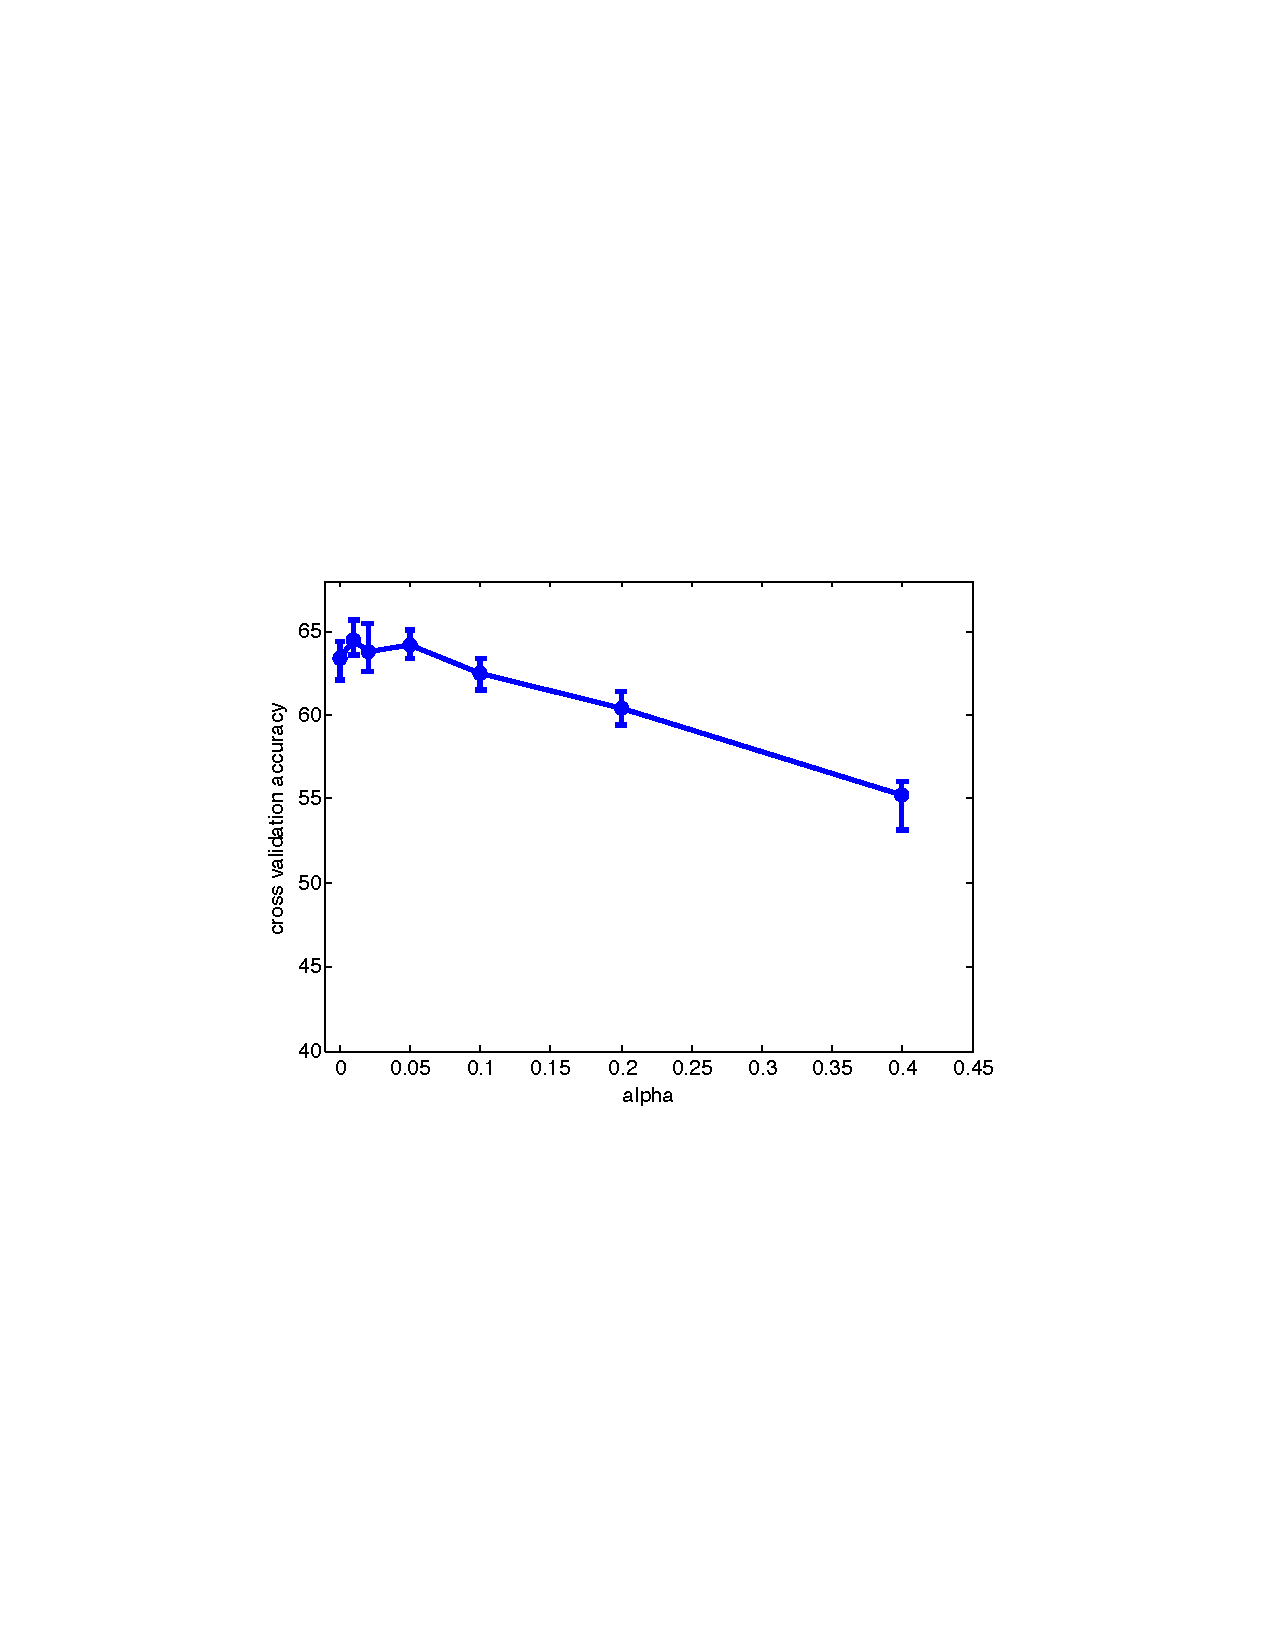
\includegraphics[width=0.45\linewidth]{alpha_plot.pdf}
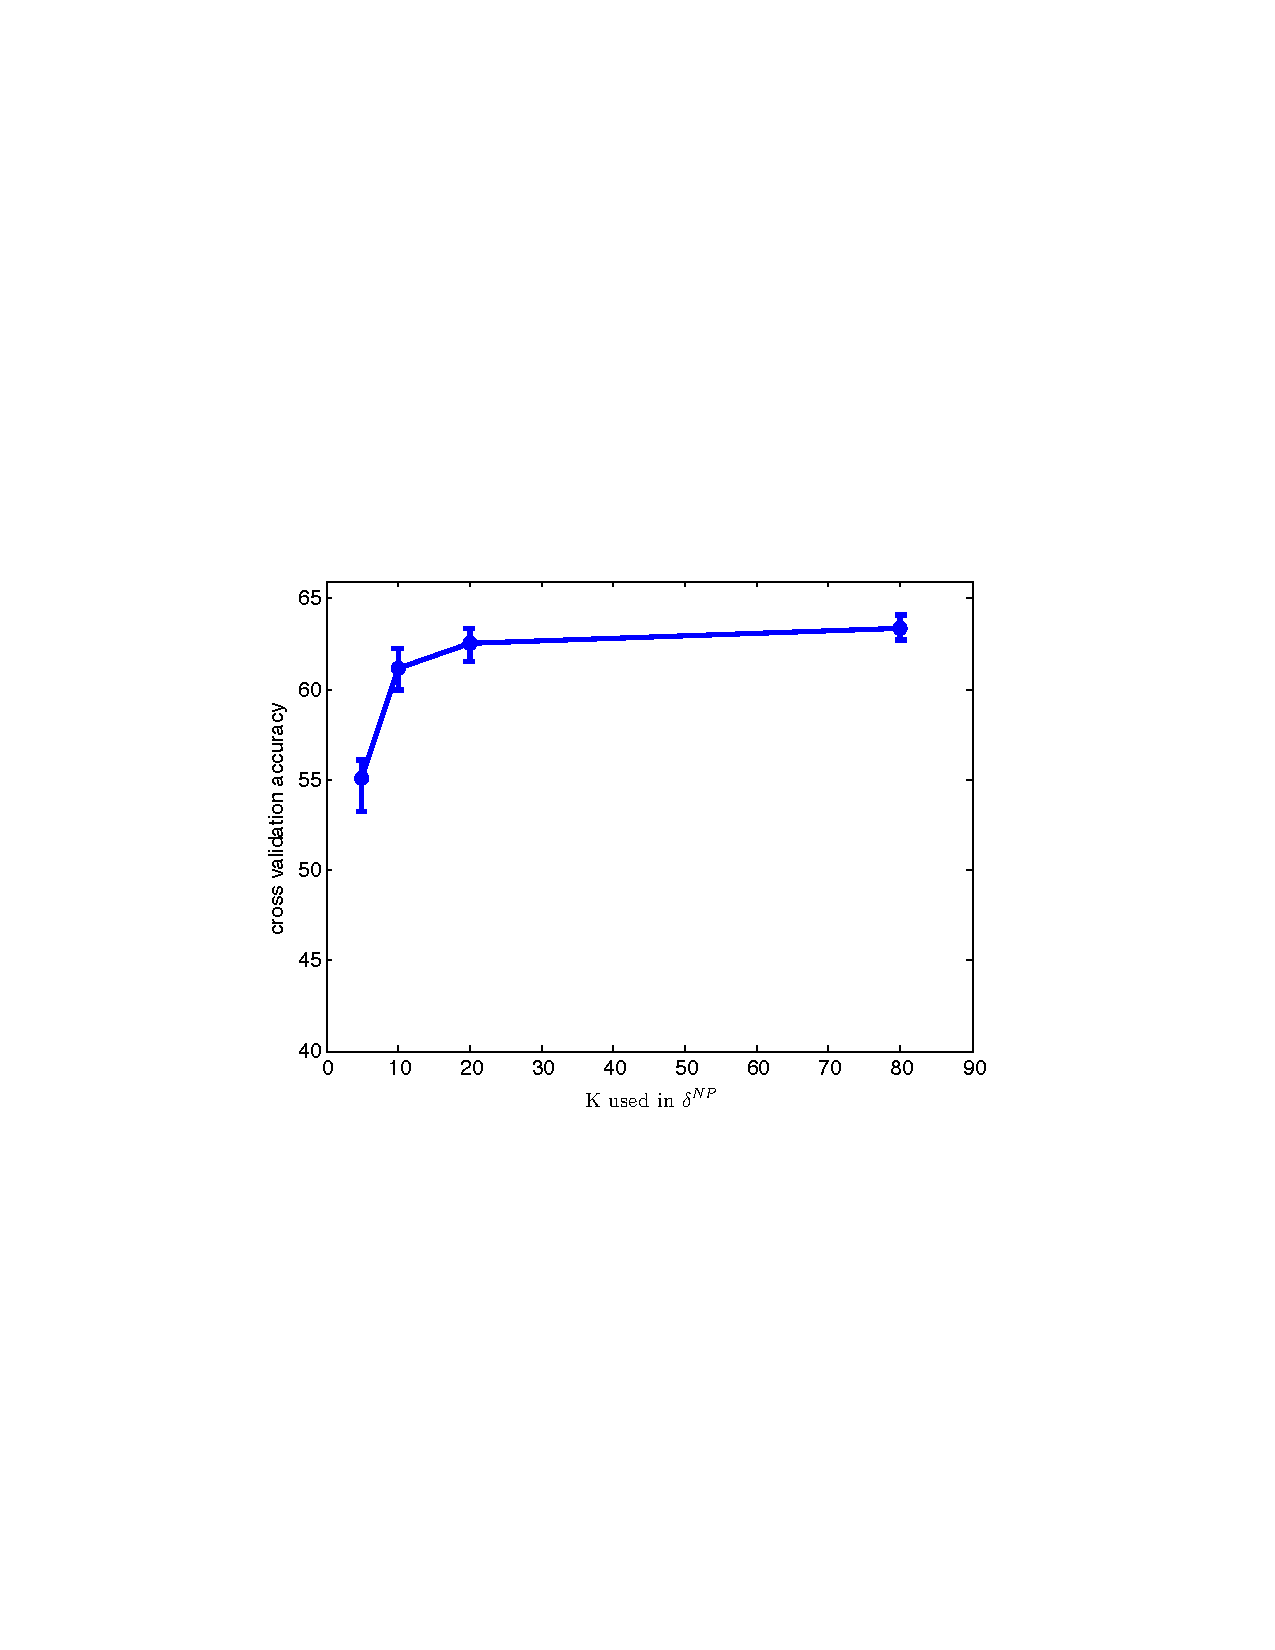
\includegraphics[width=0.45\linewidth]{K_plot.pdf}
\end{center}
\caption{Cross-validation results on fine-grained accuracy for different values of $\alpha$ (left) and $K$ (right). We split the training data into 5 folds and use cross-validate each hyperparameter setting.}
\label{fig:crossvalidationalphak}
\end{figure*}




As shown in Table \ref{tab:partlocalres}, for both settings of given bounding box and unknown bounding box, our methods outperform the strong DPM~\cite{Hossein_ECCV12} method.
Adding a geometric constraint $\delta^{NP}$ improves our results (79.82\% for body localization compared to 65.42\%). In the fully automatic setting, the top ranked detection and part localization performance on head is 65\% better than the baseline method. $\Delta_{\mathrm{null}}=1$ is the appearance-only case with no geometric constraints applied. Although the fine-grained classification results don't show a big gap between $\Delta_{\mathrm{geometric}}$ and $\Delta_{\mathrm{box}}$, we can see the performance gap for part localization.
The reason for the small performance gap might be that deep convolutional features are invariant to small translations and rotations,
limiting the impact of small localization errors on our end-to-end accuracy.


We also evaluate the recall performance of selective search region proposals \cite{selsearch} for bounding box and semantic parts. 
The results of recall given different overlapping thresholds are shown in Table \ref{tab:selective_search_recall}. 
Recall for the bird head and body parts is high when the overlap requirement is $0.5$, which provides the foundation for localizing these parts given the region proposals. However, we also observe that the recall for head is below $40\%$ when the overlap threshold is $0.7$, indicating the bottom-up region proposals could be a bottleneck for precise part localization.

Other visualizations are shown in Figure~\ref{fig:comparasion}. We show three detection and part localization for each image, the first column is the output from strong DPM, the second column is our methods with individual part predictions and the last column is our method with local prior. We used the model pretrained from \cite{Hossein_ECCV12} to get the results. We also show some failure cases of our method in Figure~\ref{fig:failure}.


\subsection{Component Analysis}
To examine the effect of different values of $\alpha$ and $K$ used in $\Delta_{\mathrm{geometric}}$, we conduct cross-validation experiments.
Results are shown in Figure~\ref{fig:crossvalidationalphak}. We fix $K=20$ in Figure~\ref{fig:crossvalidationalphak}, left and fix $\alpha = 0.1$ in Figure \ref{fig:crossvalidationalphak}, right. All the experiments on conducted on training data in a cross-validation fashion and we split the training data into 5 folds.
%\todo{can we add error bars? ... if you still have the results}.
As the results show, the end-to-end fine-grained classification results are sensitive to the choice of $\alpha$ and $\alpha=0$ is the case of $\Delta_{\mathrm{box}}$ predictions without any geometric constraints. The reason why we have to pick a small $\alpha$ is the pdf of the Gaussian is large compared to the logistic score function output from our part detectors. On the other hand, the choice of $K$ cannot be too small and it is not very sensitive when $K$ is larger than 10. 


%Experiment results vary K, vary $\alpha$
%Answer the following questions,
%1) Are parts necessary, show results with only root filter
%2) Are neighbors necssarcy, show only fit into one Gaussian
%3) Show hor prior helps, show results without prior
%
%figure to visualize the prior over neighbors v.s. prior over the whole training data


\begin{figure*}
\begin{center}
\begin{tabular}{ccc}
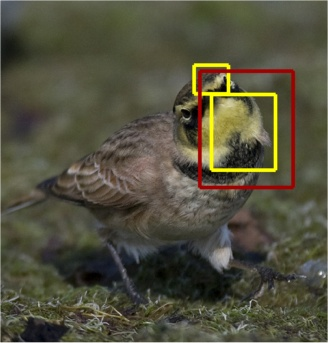
\includegraphics[width=0.3\linewidth]{6_strong_dpm.jpg} &
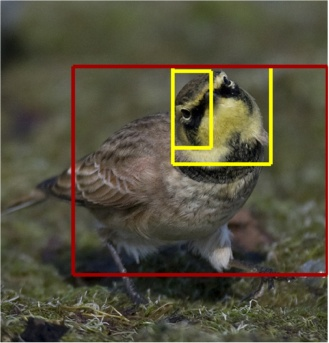
\includegraphics[width=0.3\linewidth]{6_individual.jpg} &
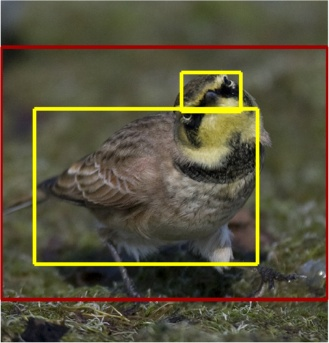
\includegraphics[width=0.3\linewidth]{6_neighbor.jpg} \\
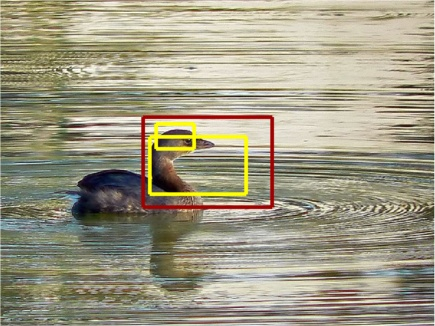
\includegraphics[trim=0mm 10mm 0mm 10mm, clip, width=0.3\linewidth]{11_strong_dpm.jpg} &
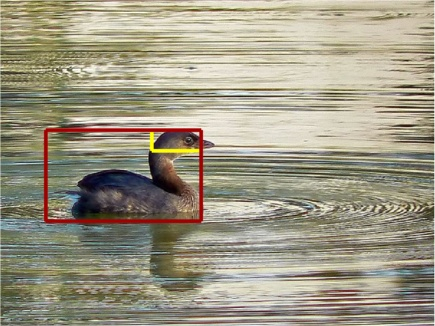
\includegraphics[trim=0mm 10mm 0mm 10mm, clip, width=0.3\linewidth]{11_individual.jpg} &
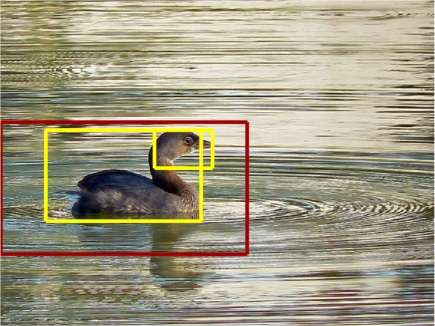
\includegraphics[trim=0mm 10mm 0mm 10mm, clip, width=0.3\linewidth]{11_neighbor.jpg} \\
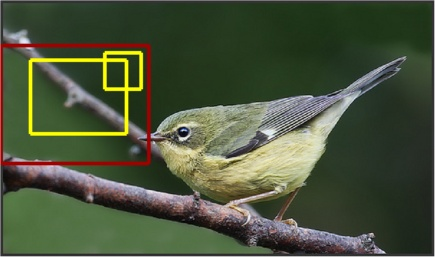
\includegraphics[width=0.3\linewidth]{13_strong_dpm.jpg} &
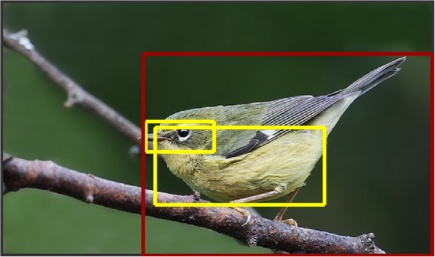
\includegraphics[width=0.3\linewidth]{13_individual.jpg} &
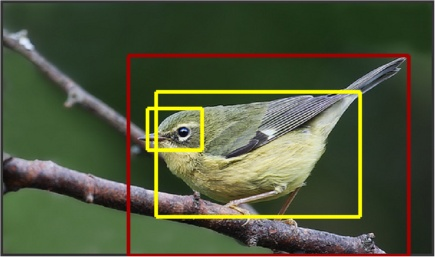
\includegraphics[width=0.3\linewidth]{13_neighbor.jpg} \\
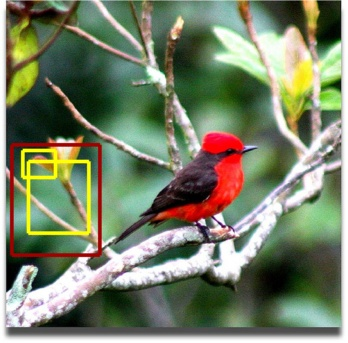
\includegraphics[trim=0mm 20mm 0mm 20mm, clip, width=0.3\linewidth]{15_strong_dpm.jpg} &
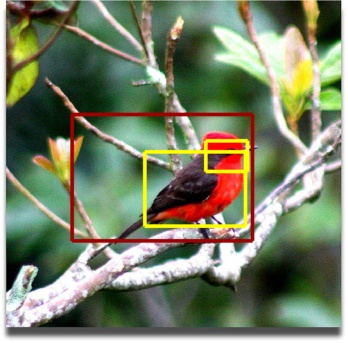
\includegraphics[trim=0mm 20mm 0mm 20mm, clip, width=0.3\linewidth]{15_individual.jpg} &
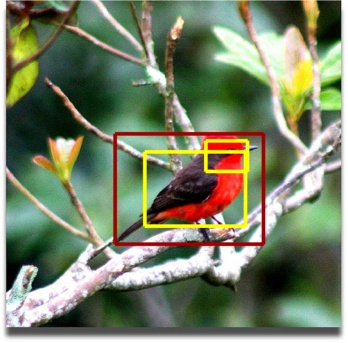
\includegraphics[trim=0mm 20mm 0mm 20mm, clip, width=0.3\linewidth]{15_neighbor.jpg} \\
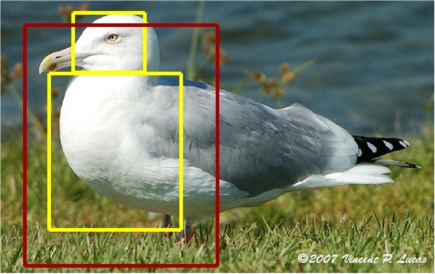
\includegraphics[width=0.3\linewidth]{16_strong_dpm.jpg} &
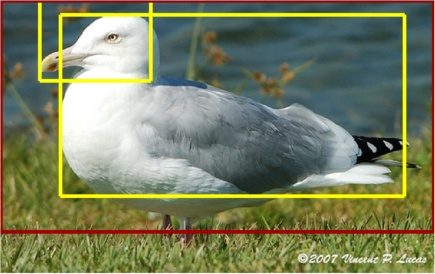
\includegraphics[width=0.3\linewidth]{16_individual.jpg} &
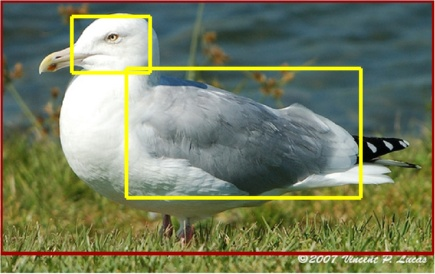
\includegraphics[width=0.3\linewidth]{16_neighbor.jpg} \\
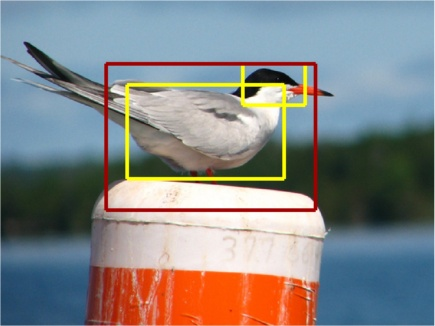
\includegraphics[width=0.3\linewidth]{17_strong_dpm.jpg} &
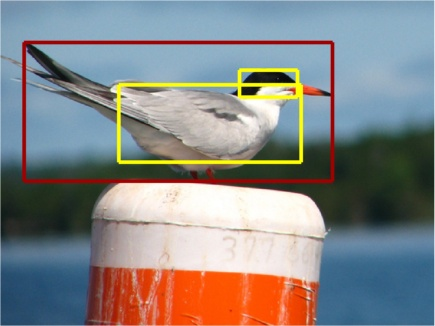
\includegraphics[width=0.3\linewidth]{17_individual.jpg} &
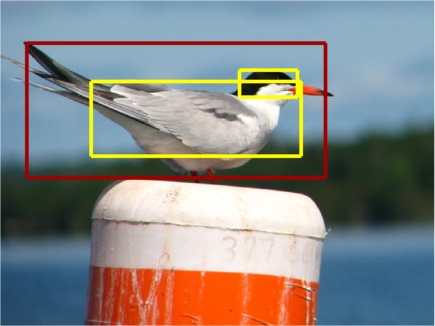
\includegraphics[width=0.3\linewidth]{17_neighbor.jpg} \\
% 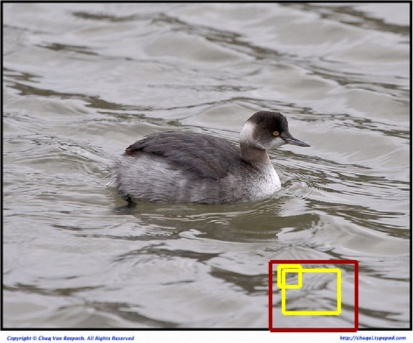
\includegraphics[width=0.3\linewidth]{19_strong_dpm.jpg} &
% 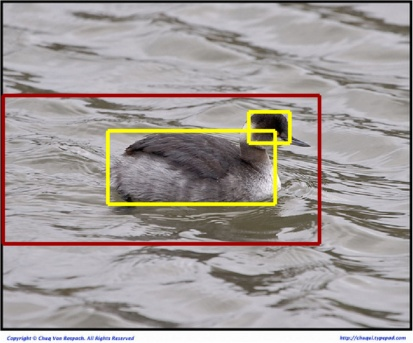
\includegraphics[width=0.3\linewidth]{19_individual.jpg} &
% 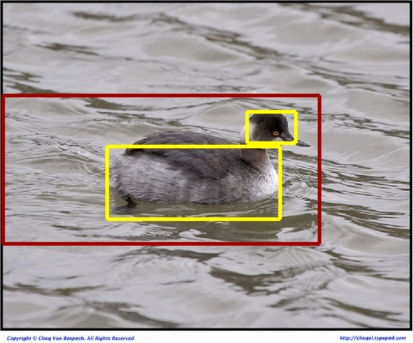
\includegraphics[width=0.3\linewidth]{19_neighbor.jpg} \\
% 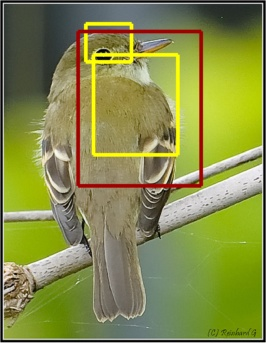
\includegraphics[width=0.3\linewidth]{30_strong_dpm.jpg} &
% 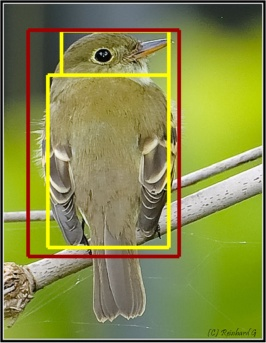
\includegraphics[width=0.3\linewidth]{30_individual.jpg} &
% 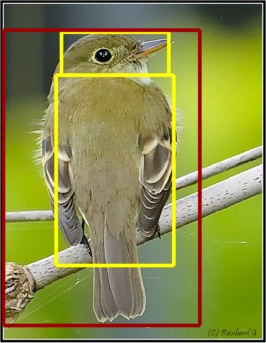
\includegraphics[width=0.3\linewidth]{30_neighbor.jpg} \\
Strong DPM & Ours ($\Delta_{box}$) & Ours ($\delta^{NP}$)
\\
\end{tabular}
\end{center}
\caption{{Examples of bird detection and part localization from strong DPM~\cite{Hossein_ECCV12} (left); our method using $\Delta_{\mathrm{box}}$ part predictions (middle); and our method using $\delta^{NP}$(right). All detection and localization results without any assumption of bounding box. }}
\label{fig:comparasion}
\end{figure*}

\begin{figure*}
\begin{center}
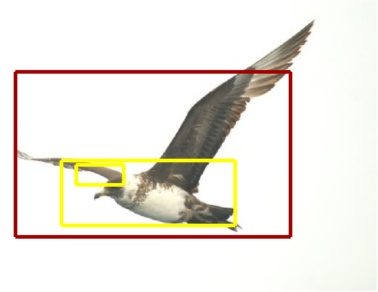
\includegraphics[height=0.2\linewidth]{8_neighbor.jpg} 
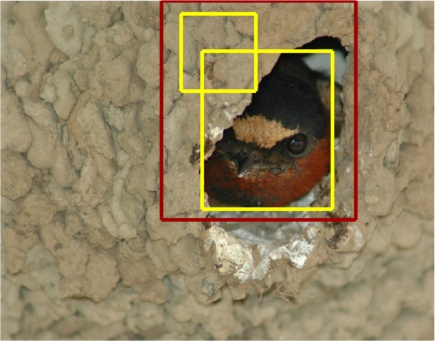
\includegraphics[height=0.2\linewidth]{32_neighbor.jpg} 
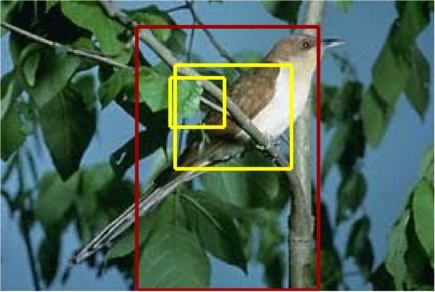
\includegraphics[height=0.2\linewidth]{41_neighbor.jpg} 
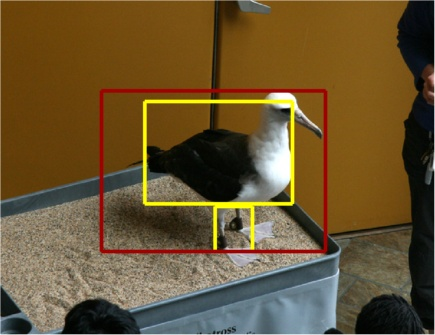
\includegraphics[height=0.2\linewidth]{57_neighbor.jpg} 
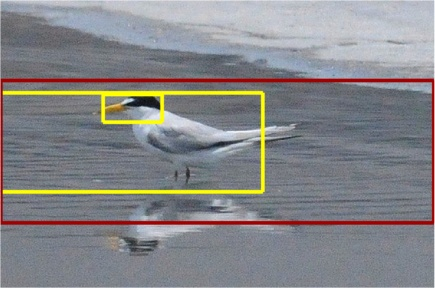
\includegraphics[height=0.2\linewidth]{58_neighbor.jpg}
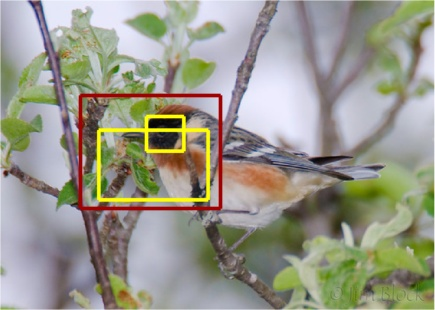
\includegraphics[height=0.2\linewidth]{64_neighbor.jpg} 
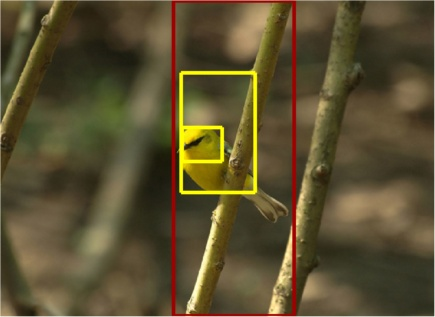
\includegraphics[height=0.2\linewidth]{99_neighbor.jpg} 
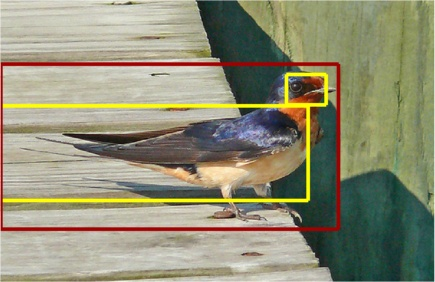
\includegraphics[height=0.2\linewidth]{47_neighbor.jpg} 
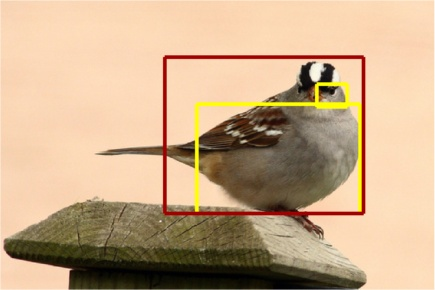
\includegraphics[height=0.2\linewidth]{91_neighbor.jpg} 
\end{center}
\caption{{Failure cases of our part localization using $\delta^{NP}$.}}
\label{fig:failure}
\end{figure*}

\section{Related work}\label{s:related}

\begin{figure}[t]
\centering
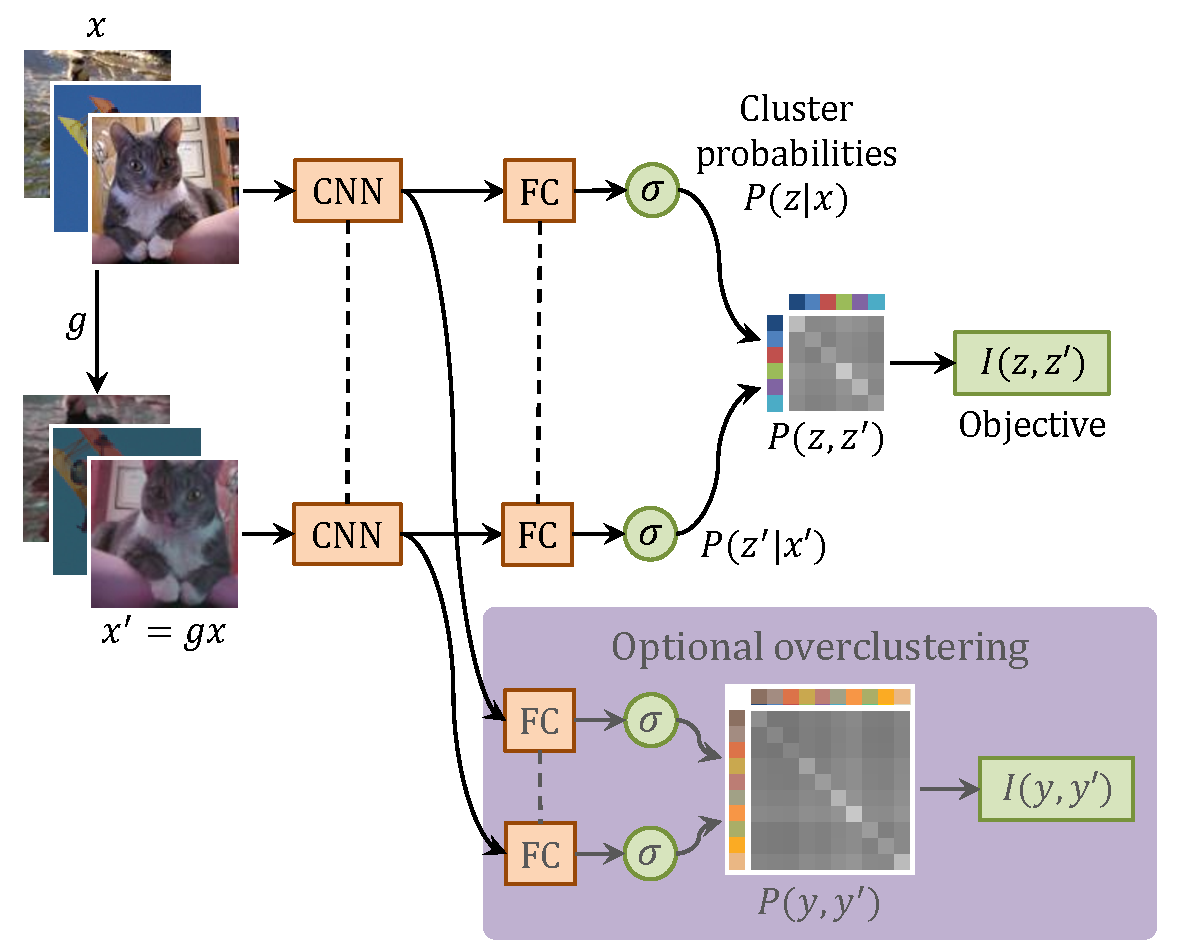
\includegraphics[width=0.95\columnwidth]{paper_imgs/overview1.pdf}
\caption{\label{f:overview}\methodnameshort for image clustering. Dashed line denotes shared parameters, $g$ is a random transformation, and $I$ denotes mutual information~(\cref{e:loss_expanded}).}
\end{figure}


\begin{figure*}
%\captionsetup{justification=centering}
\setlength\tabcolsep{2.2pt} % default value: 6pt

\begin{tabular}{c c c c c c}
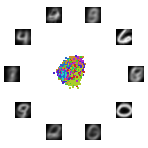
\includegraphics[height=0.16\textwidth]{experiments2_files/mnist_progression/726_run_1_colour_0_pointcloud_0.png} & 
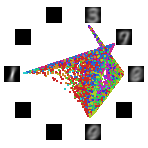
\includegraphics[height=0.16\textwidth]{experiments2_files/mnist_progression/726_run_1_colour_0_pointcloud_3.png} & 
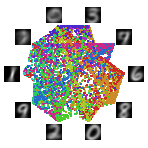
\includegraphics[height=0.16\textwidth]{experiments2_files/mnist_progression/726_run_1_colour_0_pointcloud_10.png} & 
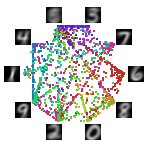
\includegraphics[height=0.16\textwidth]{experiments2_files/mnist_progression/726_run_1_colour_0_pointcloud_30.png} & 
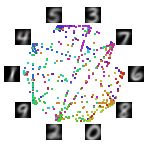
\includegraphics[height=0.16\textwidth]{experiments2_files/mnist_progression/726_run_1_colour_0_pointcloud_101.png} & 
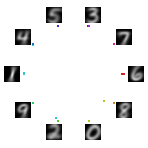
\includegraphics[height=0.16\textwidth]{experiments2_files/mnist_progression/726_run_1_colour_0_pointcloud_1000.png} 
\end{tabular}

\caption{\label{f:mnist_dots} Training with \methodnameshort on unlabelled MNIST in successive epochs from random initialisation (left). The network directly outputs cluster assignment probabilities for input images, and each is rendered as a coordinate by convex combination of 10 cluster vertices. There is no cherry-picking as the entire dataset is shown in every snapshot. Ground truth labelling (unseen by model) is given by colour. At each cluster the average image of its assignees is shown. With neither labels nor heuristics, the clusters discovered by \methodnameshort correspond perfectly to unique digits, with one-hot certain prediction (right).}
\end{figure*}


\paragraph{Co-clustering and mutual information.}

The use of information as a criterion to learn representations is not new. One of the earliest works to do so is by Becker and Hinton~\cite{becker1992self}.
More generally, learning from paired data has been explored in co-clustering~\cite{hartigan1972direct, dhillon2003information} and in other works~\cite{wang2010information} that build on the information bottleneck principle~\cite{friedman2001multivariate}.

Several recent papers have used information as a tool to train deep networks in particular.
IMSAT~\cite{hu2017learning} maximises mutual information between data and its representation and DeepINFOMAX~\cite{hjelm2018learning} maximizes information between spatially-preserved features and compact features.
However, IMSAT and DeepINFOMAX combine information with other criteria, whereas in our method information is the only criterion used.
Furthermore, both IMSAT and DeepINFOMAX compute mutual information over continuous random variables, which requires complex estimators~\cite{belghazi2018mine}, whereas \methodnameshort does so for discrete variables with simple and exact computations.
Finally, DeepINFOMAX considers the information $I(\bx, f(\bx))$ between the features $\bx$ and a deterministic function $f(\bx)$ of it, which is in principle the same as the entropy $H(\bx)$; in contrast, in \methodnameshort information does not trivially reduce to  entropy.

\paragraph{Semantic clustering versus intermediate representation learning.}
In semantic clustering, the learned function directly outputs discrete assignments for high level (i.e. semantic) clusters. Intermediate representation learners, on the other hand, produce continuous, distributed, high-dimensional representations that must be post-processed, for example by k-means, to obtain the discrete low-cardinality assignments required for unsupervised semantic clustering. The latter includes objectives such as generative autoencoder image reconstruction~\cite{vincent2010stacked},  triplets~\cite{schultz2004learning} and spatial-temporal order or context prediction~\cite{lee2017unsupervised,cruz2017deeppermnet,doersch2015unsupervised}, for example predicting patch proximity~\cite{isola2015learning}, solving jigsaw puzzles~\cite{noroozi2016unsupervised} and inpainting~\cite{pathak2016context}. Note it also includes a number of clustering methods (DeepCluster~\cite{caron2018deep}, exemplars~\cite{dosovitskiy2015discriminative}) where the clustering is only auxiliary; a clustering-style objective is used but does not produce groups with semantic correspondence. For example, DeepCluster~\cite{caron2018deep} is a state-of-the-art method for learning highly-transferable intermediate features using overclustering as a proxy task, but does not automatically find semantically meaningful clusters. As these methods use auxiliary objectives divorced from the semantic clustering objective, it is unsurprising that they perform worse than \methodnameshort~(\cref{s:experiments}), which directly optimises for it, training the network end-to-end with the final clusterer implicitly wrapped inside.




\paragraph{Optimising image-to-image distance.}

Many approaches to deep clustering, whether semantic or auxiliary, utilise a distance function between input images that approximates a given grouping criterion.
Agglomerative clustering~\cite{bautista2016cliquecnn} and partially ordered sets~\cite{bautista2017deep} of HOG features~\cite{dalal2005histograms} have been used to group images, and exemplars~\cite{dosovitskiy2015discriminative} define a group as a set of random transformations applied to a single image. Note the latter does not scale easily, in particular to image segmentation where a single $200\times 200$ image would call for 40k classes. DAC~\cite{chang2017deep}, JULE~\cite{yang2016joint}, DeepCluster~\cite{caron2018deep}, ADC~\cite{haeusser2018associative} and DEC~\cite{xie2016unsupervised} rely on the inherent visual consistency and disentangling properties~\cite{greff2015binding} of CNNs to produce cluster assignments, which are processed and reinforced in each iteration. 
The latter three are based on k-means style mechanisms to refine feature centroids, which is prone to degenerate solutions~\cite{caron2018deep} and thus needs explicit prevention mechanisms such as pre-training, cluster-reassignment or feature cleaning via PCA and whitening~\cite{xie2016unsupervised, caron2018deep}.

\begin{comment}
DAC is the only unsupervised clustering algorithm out of these that eschews k-means and agglomerative clustering for a different but similar clustering scheme, based on feature inner-products rather than distances.
DAC forms clusters gradually, in a self-paced manner, thus alleviating but not eliminating the risk of incurring degenerate solutions.
Furthermore, the nature of the optimisation, which reinforces bootstrapped class labels, creates a strong dependency on initialisation.

For unsupervised feature learning in general, i.e.\ where the training objective is not clustering, a large number of works explore using proxy learning tasks. 
There are two major directions:  generative tasks such as autoencoder image reconstruction~\cite{vincent2010stacked}, and spatial-temporal order or context prediction~\cite{lee2017unsupervised,cruz2017deeppermnet,doersch2015unsupervised}. The latter includes predicting patch proximity~\cite{isola2015learning}, solving jigsaw puzzles~\cite{noroozi2016unsupervised} and inpainting~\cite{pathak2016context}. 
In many cases they benefit from principled formulations that protect against degeneracy.
However, unlike the aforementioned clustering methods, the features learned by these methods need to be post-processed, for example using k-means, to cluster the data. 

\end{comment}

\paragraph{Invariance as a training objective.}

Optimising for function outputs to be persistent through spatio-temporal or non-material distortion is an idea shared by \methodnameshort with several works, including exemplars~\cite{dosovitskiy2015discriminative}, IMSAT~\cite{hu2017learning}, proximity prediction~\cite{isola2015learning}, the denoising objective of Tagger~\cite{greff2016tagger}, temporal slowness constraints~\cite{zou2012deep}, and optimising for features to be invariant to local image transformations~\cite{sohn2012learning,hui2013direct}.
More broadly, the problem of modelling data transformation has received significant attention in deep learning, one example being the transforming autoencoder~\cite{hinton2011transforming}.


% \section{Related work}\label{s:related}

% \paragraph{Co-clustering and mutual information.}

% The idea of learning a data representation by seeking the common parts of related observations is not new. 
% An early work is Becker and Hinton~\cite{becker1992self}, which maximises agreement between representations of 2D images to learn depth, using an objective corresponding to maximising mutual information between the input and the average of the data representations. 
% Co-learning has also been explored in the context of clustering by co-clustering methods, dating back to the pioneering work of Hartigan~\cite{hartigan72direct}. 
% Many information-theoretic variant of such approaches have been proposed, as discussed by~\cite{wang10information}, which are generally related to the information bottleneck principle~(\cite{friedman2001multivariate}). 

% A few works have employed mutual information in the context of unsupervised deep learning. IMSAT~\cite{hu2017learning} maximises mutual information between input data and their predicted discrete representations whilst encouraging the representations of augmented data points to be close to those of the original data points. 
% DeepINFOMAX~\cite{hjelm2018learning} maximises mutual information between spatially preserved features and compact features. There are some major differences with \methodnameshort. 
% Firstly, mutual information is used as an aid in these methods, as it increases the statistical predictivity between two random variables. 
% This contrasts with our method, where mutual information constitutes the loss applied directly to cluster assignments, meaning it is used as a clustering objective. 
% Secondly, both IMSAT and DeepINFOMAX compute mutual information over continuous random variables, which calls for an integral and is not computationally tractable, so estimators~\cite{belghazi2018mine} are used. 
% Since \methodnameshort maximises mutual information between cluster assignments and the number of clusters is discrete, computation is exact and straightforward. 
% Finally, DeepINFOMAX employs mutual information between function inputs and outputs, i.e. $I(x, f(x))$, but the conditional entropy component of mutual information $H(f(x) | x)$ is 0 when $f$ is deterministic, making the maximisation less meaningful. 
% In contrast \methodnameshort maximises mutual information between cluster assignments of separate images, i.e. $I(z, z')$ where $z$ and $z'$ are not functions of one other, making $H(z | z')$ a non-zero quantity that contributes to the optimisation as it can be minimised.

% \paragraph{Optimising image-to-image distance for clustering.}
% Many works for on unsupervised deep clustering involve establishing a scheme for estimating the semantic distance between input images, before training a function to learn this scheme. 
% CliqueCNN~\cite{bautista2016cliquecnn} trains a network to discriminate between cliques that are determined by applying agglomerative clustering on image features such as HOG~\cite{dalal2005histograms}. 
% In Exemplar CNNs~\cite{dosovitskiy2016discriminative}, each image and a its set of random transformations is considered a class, and a function is trained to discriminate between these surrogate classes. Like \methodnameshort, this method uses random transformations as a proxy for obtaining images with low semantic distance in the absence of label information. 
% Requiring one class per input image has a large memory footprint which makes Exemplar CNNs infeasible for segmentation (where patches are clustered instead of images, so a single 200x200 image would call for 40k classes). 

% \begin{figure}[t]
\centering
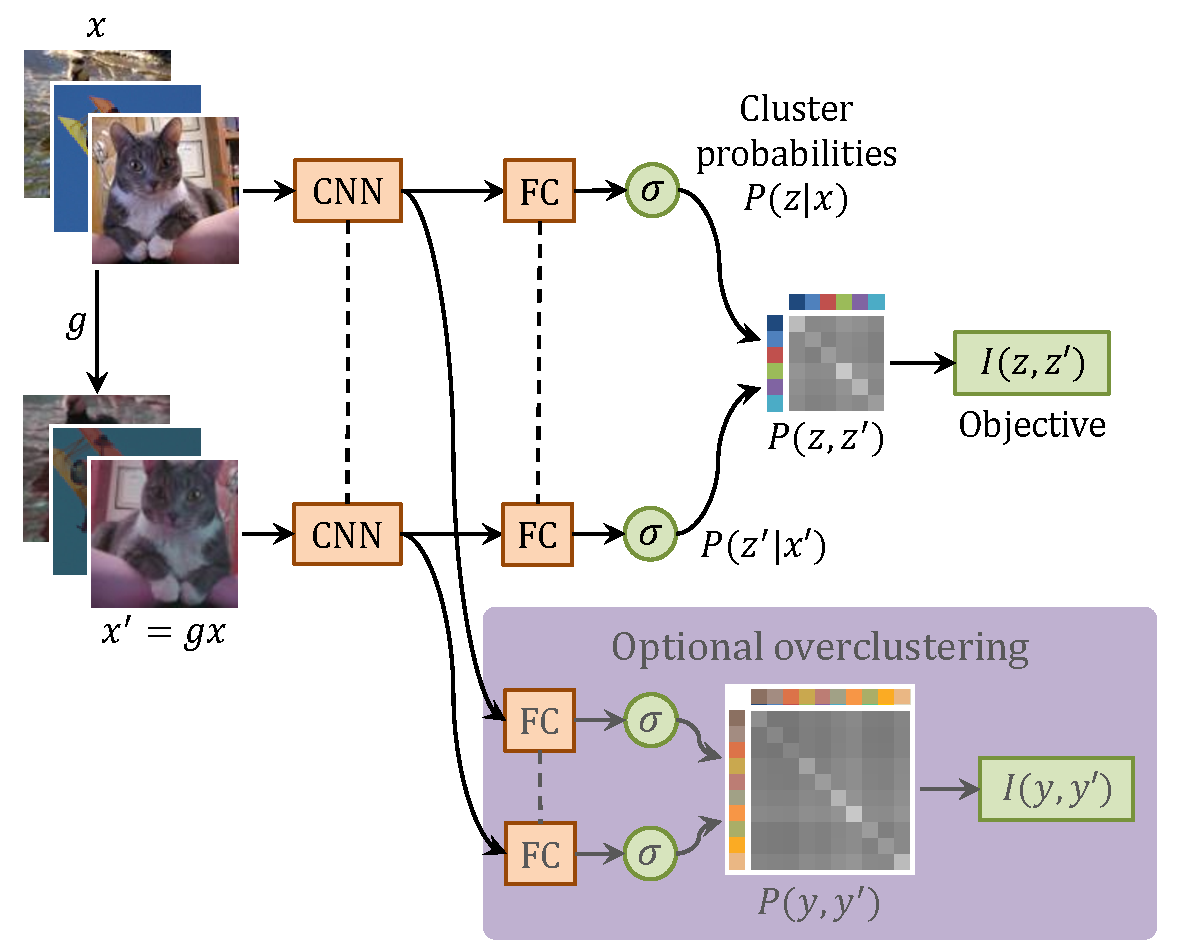
\includegraphics[width=0.95\columnwidth]{paper_imgs/overview1.pdf}
\caption{\label{f:overview}\methodnameshort for image clustering. Dashed line denotes shared parameters, $g$ is a random transformation, and $I$ denotes mutual information~(\cref{e:loss_expanded}).}
\end{figure}


% DAC~\cite{chang2017deep}, JULE~\cite{yang2016joint}, DeepCluster~\cite{caron2018deep}, Associative Deep Clustering~\cite{haeusser18associative} and DEC~\cite{xie2016unsupervised} all rely on the inherent visual consistency and disentangling properties~\cite{greff2015binding} of CNNs to produce meaningful cluster assignments, which are processed and reinforced in each iteration. 
% The latter three are based on using k-means to refine deep feature vectors, a mechanism which is prone to degenerate solutions~\cite{caron2018deep} and thus needs explicit prevention mechanisms such as pre-training, cluster-reassignment or feature cleaning via PCA and whitening ~\cite{xie2016unsupervised, caron2018deep}. 

% DAC is the only unsupervised clustering algorithm out of these that eschews k-means whilst training a network to directly produce cluster assignments, as \methodnameshort does. 
% A network is trained to produce cluster assignment probability distributions for each sample that are used as high level feature descriptors, and the dot product of different descriptors is treated as a proxy for inter-sample semantic distance (instead of Euclidian distance, which is used in the k-means based clusterers). 
% Training proceeds by maximising the dot product of close sample pairs, thus encouraging them to be assigned to the same cluster, whilst minimising the dot product for far pairs. 
% The nature of the optimisation means there is a strong dependency on initialisation and lack of protection against degenerate solutions such as clusters disappearing. 

% \paragraph{Proxy tasks for unsupervised feature learning.}
% For unsupervised feature learning in general, i.e. where the training objective is not clustering, a large number of works explore using proxy learning tasks. 
% There are two major camps:  generative tasks such as autoencoder image reconstruction~\cite{vincent2010stacked}, and spatial-temporal order or context prediction~\cite{lee2017unsupervised,cruz2017deeppermnet,doersch2015unsupervised}. The latter includes predicting patch proximity~\cite{isola2015learning}, solving jigsaw puzzles~(\cite{noroozi2016unsupervised}) and inpainting~(\cite{pathak2016context}). 
% In many cases they benefit from principled formulations that protect against degeneracy.
% However, unlike the aforementioned clustering methods, learned representations from these tasks constitute fine-grained continuous features rather than coarse cluster assignments, and thus must be post-processed, either by unsupervised clustering such as k-means or with label information via SVMs or fine-tuning, in order to produce semantic clusters.

% \paragraph{Invariance as a training objective.}
% Training for function outputs to be persistent through spatio-temporal distortion, noise distortion, or random transforms is an idea shared by \methodnameshort and several mentioned works, including Exemplar CNNs~\cite{dosovitskiy2016discriminative}, IMSAT~\cite{hu2017learning} and proximity prediction~\cite{isola2015learning}.
% It is also seen in Tagger~\cite{greff2016tagger}, which trains a function to denoise its input using several clusters to distribute the representation,~\cite{zou2012deep} which enforces a temporal slowness constraint on learned features, and~\cite{sohn2012learning,hui2013direct} which train for features invariant to local image transformations.



\section{Conclusions}

% We propose a novel architecture, Transformer-XL, for language modeling with self-attention architectures beyond a fixed-length context. 
Transformer-XL obtains strong perplexity results, models longer-term dependency than RNNs and Transformer, achieves substantial speedup during evaluation, and is able to generate coherent text articles. We envision interesting applications of Transformer-XL in the fields of text generation, unsupervised feature learning, image and speech modeling.





\subsubsection*{Acknowledgments}
This work was supported by the DARPA award D17AP00001, the Google focused award, and the Nvidia NVAIL award.

%
%Use unnumbered third level headings for the acknowledgments. All
%acknowledgments, including those to funding agencies, go at the end of the paper.

\clearpage

\bibliography{iclr2018_conference}
\bibliographystyle{iclr2018_conference}

\clearpage
%%%%%%%%%%%%%%%%%%%%%%%%%%%%%%%%%%%%%%%%%%%%%%%%%%%%%%%%%%%%%%
%%%%%%%%%%%%%%%%%%%% APPENDIX %%%%%%%%%%%%%%%%%%%%%%%%%%%%%%
%%%%%%%%%%%%%%%%%%%%%%%%%%%%%%%%%%%%%%%%%%%%%%%%%%%%%%%%%%%%%%

\appendix

%\section*{Appendix}

\section{Additional Details on Multi-Scale Processing}
\label{app:detailsMultiscale}

The integration of multi-scale parallel pathways in architectures that use solely unary kernel strides, such as the proposed, was described in Sec.~\ref{subsec:multiscaleCnn}. The required up-sampling of the low-resolution features was performed with simple repetition in our experiments. This was found sufficient, with the following hidden layers learning to combine the multi-scale features. In the case of architectures with strides greater than unary, the last convolutional layers of the two pathways, $L1$ and $L2$, have receptive fields $\boldsymbol{\varphi}_{L1}$ and $\boldsymbol{\varphi}_{L2}$ with strides $\boldsymbol{\tau}_{L1}$ and $\boldsymbol{\tau}_{L2}$ respectively. To preserve spatial correspondence of the multi-scale features and enable the network for dense inference, the dimensions of the input segments should be chosen such that the FMs in $L2$ can be brought to the dimensions of the FMs in $L1$ after sequential resampling by $\uparrow \boldsymbol{\tau}_{L2}$, $\uparrow F_D$, $\downarrow \boldsymbol{\tau}_{L1}$ or equivalent combinations. Here $\uparrow$ and $\downarrow$ represent up- and down-sampling by the given factor. Because they are more reliant on these operations, utilization of more elaborate, learnt upsampling schemes (\cite{Long2014, Ronneberger2015, Noh2015}) should be beneficial in such networks.


\section{Additional Details on Network Configurations}
\label{app:detailsConfig}

\textbf{3D Networks:} The main description of our system is presented in Sec.~\ref{sec:segmentationSystem}. All models discussed in this work outside Sec.~\ref{subsec:val3dContext} are fully 3D CNNs. Their architectures are presented in Table \ref{subtab:netsConfig3d}. They all use the PReLu non-linearity (\cite{he2015delving}). They are trained using the RMSProp optimizer (\cite{rmsProp}) and Nesterov momentum (\cite{sutskever2013importance}) with value $m=0.6$. $L1 = 10^{-6}$ and $L2 = 10^{-4}$ regularisation is applied. We train the networks with dense-training on batches of 10 segments, each of size $25^3$. Exceptions are the experiments in Sec~\ref{subsec:valDenseTraining}, where the batch sizes were adjusted along with the segment sizes, to achieve similar memory footprint and training time per batch. The weights of our shallow, 5-layers networks are initialized by sampling from a normal distribution $\mathcal{N}(0,0.01)$ and their initial learning rate is set to $a=10^{-4}$. Deeper models (and the \quot{Shallow+} model in Sec~\ref{subsec:valDeeper}) use the weight initialisation scheme of \cite{he2015delving}. The scheme increases the signal's variance in our settings, which leads to RMSProm decreasing the effective learning rate. To counter this, we accompany it with an increased initial learning rate $a = 10^{-3}$. Throughout training, the learning rate of all models is halved whenever convergence plateaus. Dropout with 50\% rate is employed on the two last hidden layers of 11-layers deep models.

\textbf{2D Networks:} Table \ref{subtab:netsConfig2d} presents representative examples of 2D configurations that were employed for the experiments discussed in Sec.~\ref{subsec:val3dContext}. Width, depth and batch size were adjusted so that total required memory was similar to the 3D version of DeepMedic. Wider or deeper variants than the ones presented did not show greater performance. A possible reason is that this number of filters is enough for the extraction of the limited 2D information and that the field of view of the deep multi-scale variant is already sufficient for the application. The presented 2D models were regularized with $L1 = 10^{-8}$ and $L2 = 10^{-6}$ since they have less parameters than the 3D variants. All but Dm2dPatch were trained with momentum $m=0.6$ and initial learning rate $a = 10^{-3}$, while the rest with $m=0.9$ and $a = 10^{-2}$ as this setting increased performance. The rest of the hyper parameters are the same as for the 3D DeepMedic.

\setcounter{table}{0}    
\renewcommand\thetable{B.\arabic{table}}

\begin{table}[!h]
\centering
\scriptsize
\caption{Network architectures investigated in Sec.~\ref{sec:vaOfNetArch} and final validation accuracy achieved in the corresponding experiments. (a) 3D and (b) 2D architectures. Columns from left to right: model's name, number of parallel identical pathways and number of feature maps at each of their convolutional layers, number of feature maps at each hidden layer that follows the concatenation of the pathways, dimensions of input segment to the normal and low resolution pathways, batch size and, finally, average DSC achieved on the validation fold. Further configuration details provided in \ref{app:detailsConfig}.}
\label{tab:netsConfig}
\begin{subtable}{1.0\linewidth}
\caption{3D Network Architectures}
\label{subtab:netsConfig3d}
\begin{tabular}{@{}m{1.5cm}m{3.7cm}m{1.2cm}m{1.2cm}m{1.2cm}m{0.8cm}m{1.3cm}}
\toprule	
	               & \#Pathways: FMs/Layer       & FMs/Hidd. & Seg.Norm. & Seg.Low &B.S. & DSC(\%)    \\ \midrule
Shallow(+)         & 1: 30,40,40,50                  & -          & 25x25x25   & -        &10  & 60.2(61.7) \\
Deep(+)            & 1: 30,30,40,40,40,40,50,50      & -          & 25x25x25   & -        &10  & 00.0(64.9)  \\
BigDeep+           & 1: 60,60,80,80,80,80,100,100    & 150,150    & 25x25x25   & -        &10  & 65.2       \\
DeepMedic          & 2: 30,30,40,40,40,40,50,50      & 150,150    & 25x25x25   & 19x19x19 &10  & 66.6       \\ \bottomrule
\end{tabular}
\end{subtable}%
\vspace{10pt}
\begin{subtable}{1.0\linewidth}
\caption{2D Network Architectures}
\label{subtab:netsConfig2d}
\begin{threeparttable}
\begin{tabular}{@{}m{1.5cm}m{3.7cm}m{1.2cm}m{1.2cm}m{1.2cm}m{0.8cm}m{1.3cm}}
\toprule	
	            & \#Pathways: FMs/Layer       & FMs/Hidd. & Seg.Norm. & Seg.Low &B.S. & DSC(\%)    \\ \midrule
%Dm\_3dSeg       & 2: 30,30,40,40,40,40,50,50      & 150,150    & 25x25x17   & 19x19x17   &10 & 62.1       \\
%Dm\_2dPatch 50\% & 2: 30,30,40,40,40,40,50,50      & 150,150    & 17x17x1    & 17x17x1   &540 & 53.7       \\
Dm2dPatch*    	& 2: 30,30,40,40,40,40,50,50      & 150,150    & 17x17x1    & 17x17x1    &540 & 58.8       \\
Dm2dSeg        & 2: 30,30,40,40,40,40,50,50      & 150,150    & 25x25x1    & 19x19x1    &250 & 60.9       \\
Wider2dSeg     & 2: 60,60,80,80,80,80,100,100    & 200,200    & 25x25x1    & 19x19x1    &100 & 61.3       \\
Deeper2dSeg    & 2: 16 layers, linearly 30 to 50 & 150,150    & 41x41x1    & 35x35x1    &100 & 61.5       \\
Large2dSeg  	& 2: 12 layers, linearly 45 to 80 & 200,200    & 33x33x1    & 27x27x1    &100 & 61.3    \\ \bottomrule
\end{tabular}
\begin{tablenotes}
            \item[*] Sampling was manually calibrated to achieve similar class balance as models that are trained on image segments. Model underperformed otherwise.
\end{tablenotes}
\end{threeparttable}
\end{subtable}
\end{table}

\section{Distribution of Tumor Classes Captured in Training}
\label{app:distrTumorClassesTrain}
\setcounter{table}{0}    
\renewcommand\thetable{C.\arabic{table}} 

\hyperref[table:trainingSamplesPercBrats2015Training]{Table C.1}

\begin{table}[!h]
\centering
\scriptsize
\caption{Real distribution of the classes in the training data of BRATS 2015, along with the distribution captured by our proposed training scheme, when segments of size $25^3$ are extracted centred on the tumor and healthy tissue with equal probability. Relative distribution of the foreground classes is closely preserved and the imbalance in comparison to the healthy tissue is automatically alleviated.}
\label{table:trainingSamplesPercBrats2015Training}
\begin{tabular}{@{}lccccc@{}}
\toprule
\multicolumn{1}{c}{} & Healthy		& Necrosis 	& Edema 		& Non-Enh. 	& Enh.Core 	\\ \midrule
Real		 			& 92.42			& 0.43		& 4.87		& 1.02		& 1.27		\\
Captured				& 58.65			& 2.48		& 24.98		& 6.40		& 7.48		\\
\bottomrule
\end{tabular}
\end{table}



\end{document}
